


\section{第 3 章
基于赛马场的量化交易数据增强问题}

\section{3.1 引言}

\begin{quote}
过去几十年间，随着金融市场的全球化和资产配置需求的快速增长，量化投资策略已成为资产管理领域的核心研究方向。其中，因子投资组合优化方法因其能够系统性地利用海量历史数据和多样化资产特征，在学术界和业界都备受关注。然而，这类策略的成功实
施关键在于有效的特征提取与信息表征 。一个长期存在的挑战在
于：如何在高效降低高维多因子空间维度的同时，精准捕捉隐含金
融信息的复杂分布特征{[}32 ，33{]}。

多因素模型本质上包含大量资产特征，这往往导致高维度和大
量冗余信息。在此背景下，传统特征压缩与信息提取方法存在显
著局限性{[}34{]}
。例如，经典方法如线性主成分分析。主成分分析（PCA）难以精准捕捉金融数据中固有的复杂非线性
结构，这直接制约了模型的预测性能{[}35 ，36{]} 。与此同时，金融市场
的非平稳性和固有噪声特性进一步阻碍了特征的稳健提取，导致
模型泛化能力显著下降{[}37{]} 。因此，如何实现高效的因子降维， 同
时提升特征的表达能力和泛化能力，仍是当前亟待解决的关键问 题。
\end{quote}

深度学习方法的快速发展为解决这些挑战提供了新的见解。作
为典型的非线性降维工具， 自动编码器通过编码器和解码器的联
合训练实现了有效的数据压缩和降维，已在众多领域成功应用{[}38 ， 39{]}
。然而，在金融因子投资领域，利用自编码器对高维因子数据进
行有效压缩的同时保持信息完整性和分布特征捕捉仍存在不足。
现有研究大多聚焦于无监督特征提取，未能充分挖掘监督信息以
进一步提升特征表达和预测能力。这可能导致降维过程中关键信
息的丢失，进而影响后续预测的准确性{[}40{]} 。与此同时，生成对抗
训练方法（尤其是生成对抗网络GAN）为学习隐含数据分布提供
了强大范式{[}41{]} 。其中，瓦瑟斯坦生成对抗网络（WGAN）及其改
进版本梯度惩罚 WGAN（WGAN -GP）在建模复杂数据分布时展
现出卓越的稳定性和高质量数据生成能力{[}42 ，43{]} 。尽管在图像生
成等领域取得了成功，但关于如何有效将生成对抗网络（GANs）
整合到金融因子数据特征提取框架中的深入研究仍较为有限{[}44 ， 45{]}。

\begin{quote}
此外，注意力机制的出现使因子权重的动态分配成为因子组合
优化学术研究的前沿课题{[}46{]} 。现有研究表明，注意力机制能有效
识别并凸显因子间的差异重要性，从而提升组合预测与优化的效 能{[}47{]}
。然而，将注意力机制与复杂特征降维及分布建模相结合的系统性、紧密
集成方法， 目前在统一框架下尚未得到充分探索，因而限制了其
在实际应用中的潜力发挥。
\end{quote}

为突破上述局限，本文提出了一种创新的综合因子建模框架，该
框架整合了多编码器架构、包含多智能体对抗（MAA）知识蒸馏的
先进预训练策略， 以及基于动态注意力的信息融合技术 。具体而 言
，该框架首先为不同金融特征组构建多个专用Transformer编码
器，实现高效且专业化的高维因子数据提取与压缩，将其转化为更
紧凑且信息丰富的潜在表示。随后，框架采用三种不同的预训练策
略：通过监督重构预训练最小化解码器损失，确保降维后的特征能
准确还原原始数据，从而保持信息保真度。与此同时，我们引入了 基于 WGAN
-GP的对抗性重构预训练方法，通过将多编码器和解码
器作为生成器，利用无监督对抗训练来学习因子数据的潜在分布特
征，从而显著提升模型在未知市场环境中的泛化能力和鲁棒性。关
键在于，我们提出了一种创新的多智能体对抗（MAA）预训练策 略
，将来自多样化生成智能体（如GRU 、 LSTM 、Transformer模 型）
的知识蒸馏成果转移至多源编码器。这种创新方法通过使编码
器的特征与表现最佳的MAA智能体的高质量预测结果保持一致，引
导编码器捕捉更稳健且分布感知的潜在表征，确保对复杂金融数据
动态的全面学习。

基于从这些多样化预训练策略中学习到的稳健潜在表征，该框
架引入了一个复杂的信息融合模块。该模块通过门控融合和注意
力机制等高级技术，动态整合异构特征组表征，从而在不同因子
类别间选择性突出相关信息。对于下游金融预测任务（包括回归 分析）

\begin{quote}
在交易决策、分类和投资决策中，针对特定任务的预测模块会进
行微调。特别值得一提的是，投资决策环节采用了定制化的期望
奖励损失函数，使模型能够直接学习基于动态动作概率来最大化
实际投资回报的策略。此外，该框架整合了全面的回测与评估系
统，通过整合模型预测结果和置信度评分，实现动态多资产权重
配置策略。这套系统采用风险调整回报率等金融指标组合，结合
对投资组合动态变化和权重调整的详细分析，为实际交易表现提
供了严谨的评估依据。

本文的主要贡献如下：

1. 针对高维金融因子数据的处理，我们提出了一种创新的多编
码器网络架构。该架构通过为不同因子组量身定制特征提取
与表征学习方法，有效解决了降维与信息压缩的双重挑战，
从而精准捕捉各因子组的内在时序动态特征与规律模式。

2. 本文创新性地提出并严格评估了一系列互补的预训练策略，
包括监督重构、基于 WGAN -GP的对抗性重构，以及开创性
的多智能体对抗（MAA）知识蒸馏方法。该综合方法实现了
金融因子特征的高效压缩与深度隐式分布建模，显著提升了
学习表征的鲁棒性和泛化能力。
\end{quote}

3. 我们系统整合了基于注意力机制和门控机制的多源信息融合
技术，将其置于多任务学习框架中，并配套构建了端到端的
实验与回测流程。这种集成方法实现了因子影响的动态自适
应分配与优化，显著提升了预测精度和泛化能力，同时为金
融投资组合策略提供了严谨的评估依据。通过深入的实证分析和全面的回测验证，我们不仅证实了所提框
架在金融预测与投资组合优化中的卓越表现，更揭示了动态因素
影响与资产特征之间的内在关联，为未来资产配置研究提供了坚
实的理论与实践支撑。

本文结构安排如下：第二部分对领域内相关研究进行综述；第
三部分方法论部分详细阐述所提出的多编码器框架、信息融合机制
及先进的预训练策略；第四部分描述实验设计，并通过对比实验和
大量回测验证该方法的有效性；第五部分总结研究发现，并展望未 来研究方向。

\section{3.2 相关工作}\label{ux76f8ux5173ux5de5ux4f5c}

\begin{quote}
\emph{3.2.1. 高维因子降维与信息压缩}
\end{quote}

传统金融资产定价模型认为，只需少数因素即可解释收益率。
尽管如此，近年来学者们已发表数百种不同的所谓风险因素，形 成了被称为`
因子动物园' 的现象{[}48{]} 。过多的因子会导致模型复
杂化和多重检验问题，因此需要有效的降维和信息压缩方法来提
取核心因子信号。经典无监督方法如主成分分析（PCA）可以从
高维特征中提取潜在因子，但纯数据驱动的因子可能忽略与资产
回报密切相关的信息{[}49{]} 。为此，近年来开发了结合经济信息的降
维技术。Kelly等人提出了工具化PCA模型，将资产特征作为工具
变量引入因子提取过程，使潜在因子载荷依赖于可观测的公司特 征{[}50{]}
。在此基础上，Gu等人提出了一种非线性降维方法，即使用
自编码器架构的模型来提取条件因子结构。该方法利用神经网络通过输入资产特征和收益数据的网络模型，学习识别反映非线性
关系的潜在因素并应用无套利约束，从而显著降低模型的定价误 差{[}51{]}
。类似地，陈等人利用深度学习结合大量特征信息构建资产
定价模型。他们以无套利条件作为目标函数，通过对抗机制生成
最难定价的组合来训练模型。结果表明，在样本外数据中，该模
型获得的夏普比率和定价精度远超传统方法， 同时能自动识别主
导资产价格的关键因素{[}52{]} 。另一方面，针对'因子泛滥' 问题，
学者们提出了双套索选择等方法来检验新因子的贡献度。冯等人
通过两阶段特征选择流程有效筛除冗余因子，有望抑制因子引入
时的无谓增长{[}48{]} 。高维降维方法将金融`大数据' 中的特征信息
压缩为少量解释性复合因子，既能有效降低噪声干扰和过拟合风
险，又能显著提升资产定价模型的预测性能与稳健性。

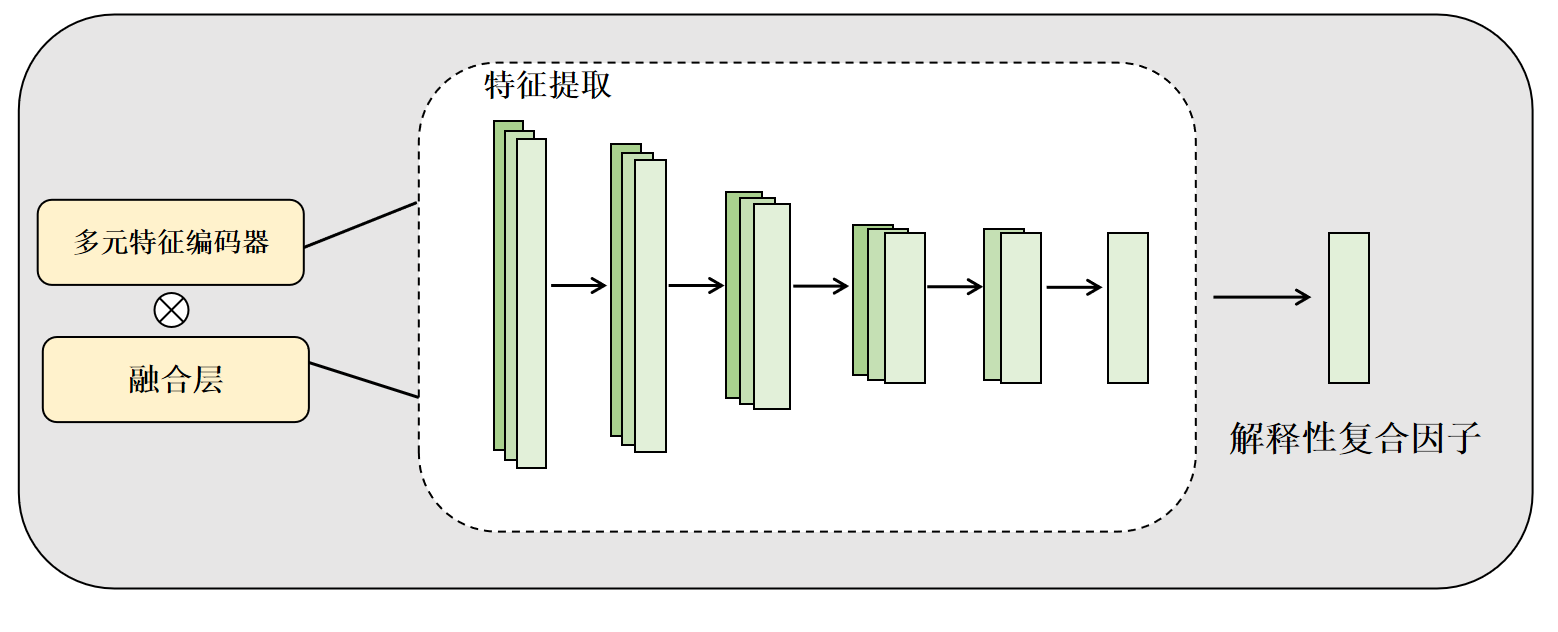
\includegraphics[width=5.76111in,height=2.33681in]{TongjiThesis-master/figures/media/image1.png}

图：高维因子降维与信息压缩任务

\begin{quote}
\emph{2.0.2. Feature Fidelity 和Supervised Reconstruction Mechanism}
\end{quote}

在高维金融数据降维领域，单纯追求方差最大化的无监督方法
可能无法保留与资产收益最相关的关键信息，导致特征表征的保
真度下降。为解决这一问题，研究者探索了结合监督信号的降维
机制，既能压缩维度又能保留原始特征中的预测信息。典型做法
是将资产收益等监督细节融入因子提取过程。例如，凯利团队开 发的 IPCA
模型本质上就是一种监督主成分分析方法。通过引入特
征对预期收益的解释力来指导因子提取， IPCA 能识别与风险溢价
密切相关的潜在因子，而非仅基于协方差贡献来选择因子。结果
显示，监督维度重新导数过程能有效保留解释收益率的特征信息{[}50{]}
。Chinco等人采用
稀疏回归（lasso）方法，从数百个候选特征中自动筛选少量预测
信号，从而实现对横截面收益率的有效预测{[}53{]} 。这种监督特征选
择方法在保持对目标变量（未来收益率）敏感性的同时，有效降
低了维度，从而提升了模型的经济意义和预测性能。近年来，深
度学习为监督重构提供了新见解。Gu等人的自动编码器因子模型
在训练过程中同时利用资产特征和收益率信息进行优化：一方面
通过神经网络编码压缩高维特征；另一方面通过解码努力重构原
始特征空间，从而确保提取的低维因子表示尽可能忠实地保留原 始信息{[}51{]}
。这种监督重构机制使模型能够在预测能力和特征完整
性之间取得平衡。实证结果表明，与传统因子模型相比，该模型
的无套利定价误差显著降低。此外，陈等人将对抗训练引入深度
定价模型，通过生成具有挑战性的场景迫使模型聚焦于真正影响
收益的因素{[}52{]} 。这一过程作为特殊形式的监督反馈，确保模型提
取的潜在因素既能有效预测收益，又保留了原始信息的异质性。
总体而言，上述方法通过整合监督信号，在保留与收益相关关键
结构的同时减少冗余噪声，从而提升降维因子对资产收益的预测
保真度，展现出更高的财务预测准确性和稳健性。

\begin{quote}
\emph{2.0.3. 潜因子分布建模的对抗训练}
\end{quote}

Goodfellow等提出的生成对抗网络（GANs）通过对抗训练在生成
器与判别器之间建立博弈关系，从而能够逼近复杂的数据分布{[}54{]} 。
近年来，金融领域已开始将对抗概念应用于风险因素与资产收益分布
的模拟建模。一方面，研究人员利用生成对抗网络（GAN）生成模拟金融数据，
以捕捉 潜在因子分布的特征。 Wiese 等人开发了Quant-GAN框
架，采用时序卷积网络（TCN）作为生成器来模拟资产对数收益
率序列。该模型能真实再现金融时间序列的统计特征（如肥尾分
布和波动性聚类）{[}55{]} 。数值测试表明，其在拟合日收益率分布和
序列依赖性方面显著优于传统 GARCH 模型，这表明对抗生成模
型能有效学习基础因子收益率的正确分布，包括极端风险尾部行
为。在资产定价与投资领域，Wang和 Chen 等人提出了
Factor-GAN框架，将GAN技术应用于多因子投资组合构建。他们利用包含70项公司特征的因子数据库，通过生成器-判别器对抗迭
代，提升了因子模型的预测准确性和稳定性。该深度因子模型在
股票收益预测能力和投资表现方面显著优于线性基准模型{[}56{]} 。更 重要的是
，对抗训练揭示了不同市场阶段中因子作用的动态变
化------例如，在国有企业改革从国有向私有过渡期间，流动性与
波动性因子的相对重要性增强，而基本面因子的影响则减弱。另
一方面，反事实思维被用于提升因子模型的稳健性。陈等人将对
抗训练机制引入深度资产定价模型：他们设计了一个生成器，持
续寻找当前模型中定价误差最显著的``难定价'' 资产组合，并将
其作为对抗训练样本。模型（判别器） 随后会针对这些最具挑战
性的投资组合进行自我调整 ，从而逼近基础因子的实际收益分
布，满足无套利条件{[}52{]} 。这种对抗训练策略能有效抑制模型对局
部模式的过度拟合，从而显著提升其识别未知风险结构的能力。
该方法为金融因子模型提供了一种创新的鲁棒化解决方案，既能
生成高度逼真的风险情景用于压力测试，又能增强模型的抗风险 能力。

\begin{quote}
该模型能够准确捕捉潜在因子分布的复杂特征。该方法在风险管
理与资产定价领域展现出显著潜力。

\emph{2.0.4. 动态因子权重分配的注意机制}
\end{quote}

注意力机制最初源自深度学习序列建模领域，其核心在于让模
型能够实时为不同输入特征分配权重，实现自适应调整{[}46{]} 。将该
机制引入金融因子模型后，可根据市场环境变化动态调整各因子
权重，从而捕捉因子效应的时变特性。传统多因子模型通常假设
因子风险溢价保持恒定，但大量研究表明，因子影响会随时间波
动并受市场环境影响。在牛市和熊市中，动量因子与价值因子等
指标的相对表现可能产生显著差异。此时，注意力机制能使模型
聚焦当前最相关的因子信号，从而实现因子权重的动态调整。近
期研究已将注意力机制融入资产定价与预测模型中。夏蒂尼团队
提出了一种注意力引导的SDF模型，该模型通过多头注意力网络识
别对随机贴现因子影响最显著的时变企业特征，其决策依据数据
驱动。引入注意力机制后，模型显著提升了定价精度。在剔除小
盘股后，注意力引导的SDF模型在解释资产横截面收益方面表现尤
为出色，且所需的投资组合权重更为平滑，从而避免了其他模型
因过度依赖小盘股提升收益而产生的极端权重现象。注意力机制
不仅提升了模型性能，还降低了交易成本（如换手率），在高市
场效率场景中表现优异{[}57{]} 。除直接将注意力机制应用于SDF外，
部分研究还将其拓展至收益预测模型。例如， 向晓团队采用自注
意力机制非线性捕捉股票特征与收益之间的复杂非线性关系，显
著提升横截面收益的预测性能{[}58{]}
。该方法的应用Transformer架构在资产定价中的应用进一步印证了注意力机制的
价值：凯利等人的研究表明，相较于传统机器学习模型，Transf-
ormer能更精准地模拟股票收益的长期依赖结构和特征交互关系，
从而显著提升资产收益的解释力和预测精度{[}59{]} 。总体而言，注意
力机制为动态因子权重配置提供了强大工具，使模型能在不同市
场环境下自主调整对关键因素的关注度， 同时弱化次要因素的影
响，从而更准确地揭示收益驱动因素。当市场波动加剧时，模型
会倾向于赋予波动性因素更高权重；反之，在市场稳定期则可能
更侧重基本面因素。这种自适应能力不仅提升了模型性能，还为
投资者提供了全新视角，帮助他们理解不同市场条件下的因子行
为，从而做出更明智灵活的资产配置决策。

\begin{quote}
\emph{2.0.5. 基于因子的资产组合优化与资产特征分析}
\end{quote}

运用因子模型指导投资组合优化是量化金融领域的核心方向之
一。虽然经典的马科维茨均值-方差理论为优化投资组合权重提供
了框架，但在实际应用中，收益和协方差的估计误差常导致最优
投资组合不稳定{[}60{]} 。将因子纳入资产配置可部分缓解这一问题，
因为因子能作为市场系统性风险和特征的代理变量，使协方差矩
阵和预期收益的估计更具稳健性，从而提升投资组合表现。Ledo-
it等人提出在多因子模型中利用因子结构估计协方差，该方法已被
证明能改善最小方差投资组合的业绩{[}61{]} 。近年来，大量研究探讨
了机器学习衍生因子在资产配置中的应用。因子投资组合通过将
具有相似定价动态的资产特征归类为复合因子，并基于这些因子
构建多头/空头投资组合，从而捕捉横截面收益并优化投资策略。
Stambaugh等学者对11种已知异常进行了分类。他们将这些因素提炼为两个独立的``
定价偏差'' 因子，结合市场和规
模因素共同构建了一个新的四因子模型，该模型能更准确地解释
广义资产组合的异常收益{[}62{]} 。这种方法表明，将众多相关特征整
合为少量因子组合，不仅简化了模型结构，还提升了资产收益的
解释力，为构建主动投资组合提供了更有效的因子基础。侯等人
提出的q因子模型以企业投资和盈利能力为核心要素，从资产供给
角度阐释股票收益，能够统一描述各类资产特征对预期收益的影
响，在实证层面比法玛-弗伦奇框架更能解释异常收益。这种由基
本面特征驱动的因子模型，为资产特征分析提供了清晰的经济直觉{[}63{]}
。在高维特征空间中，学者们已开始直接寻求最优组合权
重。科扎克等人研究团队采用贝叶斯收缩方法，从数十个候选因
子中直接构建稳健的随机贴现因子（SDFs），通过惩罚低方差成
分有效整合高维特征 。其`` 收缩横截面 '' 模型在样本外表现优
异，相较于仅使用少数已知因子的模型，能更高效地利用整个特 征空间：
即使传统的四因子或五因子模型无法完全概括所有预期
的横截面收益变化，该方法也表明只需提取少量主成分即可近似
所有特征的定价结构{[}64{]} 。与此同时，Bianchi等人对各类机器学习
因子在资产配置中的有效性进行了评估。研究发现，在构建最小
方差投资组合时，采用自编码器和稀疏方法提取的潜在因子，相较于主成分分析（PCA）等传统方法，能实现更低的投资组合波动
率和更优的风险调整回报{[}65{]} 。这表明机器学习提取的因子不仅能
解释资产收益，还可用于优化投资组合风险管理。因子驱动的投
资组合优化还深化了资产特征分析。通过聚焦投资组合对各类资
产特征的暴露程度，投资者可精准识别哪些资产特征才是真正的价值来源。

\begin{quote}
超额收益。简而言之，因子驱动的投资组合优化方法，将海量资
产特征转化为少数几个具有经济意义的因子来指导资产配置。这
种方法不仅能提升投资组合的风险调整后收益，还能帮助投资者
深入理解资产特征与投资组合表现之间的内在联系，在量化投资
实践中展现出巨大价值{[}61{]}。
\end{quote}

\section{3.3基于赛马场式多智能体对抗的高维数据增强方法：算法机制}

赛马场：在群组交叉对抗基础上，将想要提升效果的模型替换掉群组交叉对抗中表现效果最差的那一个生成器，重复群组交叉对抗的过程。基线是想要提升效果的模型。

\begin{quote}
3.3.1高维数据增强

本节详细阐述本文提出的多源特征型金融时间序列建模框架。
该框架通过为各类金融特征设计专属编码、高效整合异构信息、
采用先进预训练策略、支持下游任务灵活适配及稳健回测等创新 设计，
旨在全面提升金融市场预测的准确性与稳健性。

\emph{3.1. 多源特征集编码}
\end{quote}

金融市场数据极为复杂，通常包含大量性质各异的指标。这些
指标可以自然划分为多个逻辑组别，例如基础交易信息（如开盘 价 、 收盘价 、
成交量 ）、 技术分析指标（ 如移动平均线 、 MACD
、相对强弱指数）、市场情绪指标以及其他衍生特征。虽
然这些数据源自同一来源，但它们代表了市场行为的不同方面，
可能具有不同的内部结构和时间模式。为了更好地捕捉这些异质
特征组的内在规律，我们设计了\textbf{多源特征组编码器架构}。该架构
的核心是为所有输入特征定义的独立特征组Gm 分配专用的Transf-
ormer编码器Encoderm 。这种设计使模型能够独立学习每个特征组
的时间动态和特征表示，避免因直接混合不同性质特征而导致的
信息混淆，从而更精准地提取每个特征组中的潜在信息。每个Encoderm
都采用Transformer编码器作为其骨干网络。Transformer模型凭借其独特的自注意力机制，能够并行处理整个输
入序列并有效捕捉长距离依赖关系，这对于处理复杂且非线性的
金融时间序列数据至关重要。对于第\emph{m}个特征组的输入序列XGm \emph{∈} R
T×DGm（其中\emph{T}为序列长度，DGm为第\emph{m}个特征组的维度），其处
理流程如下：

\begin{quote}
首先，输入特征通过线性层投影到模型的潜在维度dmodel：

x \emph{,Gm ，t}=\textbf{xGm}\emph{，t} \textbf{W}输入
，\emph{m}+\textbf{b输入}，\emph{m} (1)

其中\textbf{x} \emph{,}Gm ,t 是时间步\emph{t}
时第\emph{m}个特征组的输入向量。随后，为在模型
中编码序列元素的时间顺序信息，引入了形式为正弦和余弦函数
的位置编码\emph{PE}：


\includegraphics[width=2.36504in,height=0.35405in]{TongjiThesis-master/figures/media/image2.png}

(2)
\end{quote}

其中\emph{pos}表示序列中的位置，2i和2i+1表示维度索引。这种位置编
码使模型能够理解序列中数据点之间的相对和绝对位置关系。输
入序列现在富含位置信息 ，被输入到多层Transformer编码器块
中，每个块包含多头自注意力机制和前馈神经网络。多头自注意
力机制使模型能够在不同表示子空间中同时关注序列的不同位
置，从而捕捉更丰富的时序依赖关系。最终，每个编码器Encod
erm输出其对应特征组的潜在表示hGm \emph{∈}R T×d model。

\begin{quote}
\emph{3.2. 多源特征集信息融合}

在获得各特征组的独立潜在表征后，有效整合这些异质但相互
关联的信息是提升模型整体性能的关键。如图\hyperref[bookmark42]{2}所示，该框架提供
了三种先进的信息融合策略，以适应不同的数据特征和融合要求，
旨在形成一个全面且信息丰富的联合潜在表征：
\end{quote}

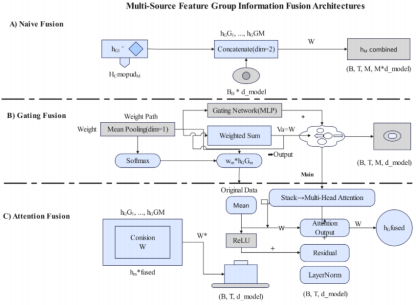
\includegraphics[width=4.32075in,height=3.17369in]{TongjiThesis-master/figures/media/image4.png}

\begin{quote}
\textbf{图2：}多源特征组信息融合架构：该图展示了如何通过三种不同的融合方
法（拼接、 门控和注意力机制）将不同特征组编码器的潜在表征进行整 合。

\emph{3.2.1. 单纯性融合}

朴素融合是最直接和基本的融合方法。它只是将所有特征组编
码器的潜在表示沿特征维度进行拼接。如果有\emph{M}个特征组，每个
特征组的潜在表示维度为dmodel ，那么融合后的组合潜在表示为
\end{quote}

hcombined \emph{∈}R T×（M·d model）。

\begin{quote}
hcombined= 连接（hG1, hG2 ，... ，\emph{hGM}） (3)

该方法高效且操作简便，适用于特征组间信息相对独立的场景，
或需保留各组完整特征以提供下游任务全面输入的情况。

3.4实验结果分析\emph{3.2.2. 门融合}

门控融合技术旨在通过动态学习为各特征组分配重要性权重，
从而实现加权自适应融合。该方法首先将所有特征组的潜在表征
进行拼接，随后通过小型门控网络（通常为多层感知器）学习生
成权重矩阵。这些权重通常采用Softmax归一化处理以确保总和为 1
，进而用于对各特征组的潜在表征进行加权求和运算。
\end{quote}

\textbf{w}= Softmax（GatingNet（Concat（hG1 , hG2 ，... ，\emph{hGM}）
\emph{·}mean（dim = 1））

\begin{quote}
) (4)

M

hfused =

\includegraphics[width=0.25084in,height=0.37625in]{TongjiThesis-master/figures/media/image5.png}\textbf{w}m
· hGm (5)

其中\textbf{w}m表示第\emph{m}个特征组的权重向量。 门控融合技术使模型能够
根据复杂多变的金融市场环境， 自适应调整对不同信息源的关注
度，从而在当前阶段突出对预测更具指导意义的特征组。

\emph{3.2.3. 注意融合}

注意力融合通过多头自注意力机制直接与特征组维度的信息交
互作用，捕捉不同特征组之间的复杂关系与交互。具体而言，将
所有特征组的潜在表征堆叠形成一个代表所有特征组（视为一 个`代理'
）的序列，随后对该序列应用多头注意力机制。

Hstacked= Stack（hG1, hG2 ，... ，\emph{hGM}） \emph{∈}R B×T×M×d 模型(6)

经过适当的维度重塑后，该模型可在特征组维度上执行注意力计
算，最终输出融合信息：

hfused= 多头注意力机制（Hstacked , Hstacked ，\emph{Hstacked}）
\emph{·}均值（维度 = 1） (7)

MultiHeadAttention技术使模型能够同时从多个角度评估特征组间
的关联性。注意力融合机制则能实现特征组间更精细、更灵活的
信息交互，尤其适用于特征组间存在复杂非线性关联或需要动态
平衡其影响的场景。

\emph{3.3. 预训练策略}
\end{quote}

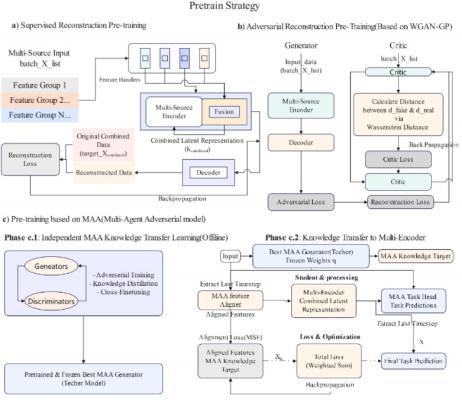
\includegraphics[width=4.80099in,height=4.17449in]{TongjiThesis-master/figures/media/image6.jpeg}

\begin{quote}
\textbf{图3：}预训练策略概述：该图展示了三种不同的预训练流程：监督重建预
训练、基于 WGAN -GP的对抗性重建预训练以及多智能体对抗（MAA）
预训练，重点说明了各自的损失函数和模型组件。

为使多源特征编码器能够学习高质量且可泛化的特征表示，需进
行三项互补的预训练
\end{quote}

如图\hyperref[bookmark43]{3}所示，研究了以下策略：监督式重构预训练、基于
WGAN -GP 的对抗性重构预训练， 以及用于知识蒸馏的多智能体对抗（MAA）
预训练。这些策略通过不同机制，从高维噪声金融数据中提取稳健且
信息丰富的潜在信息。

\begin{quote}
\emph{3.3.1. 监督重构预训练}
\end{quote}

该策略的核心思想是利用自编码器机制迫使编码器学习一个能
够准确重构原始输入数据的潜在表示。训练一个\emph{解码器}，该解码
器以多源特征编码器输出的组合潜在表示hcombined作为输入，尝试
重构原始完整输入特征$X_{original}  \in R T \times D_{total}$（其中Dtotal为所有原始特征维度的总和）
。该\emph{解码器}还采用Transformer主干网络，其任务是最小化重构误差：

\begin{quote}

\includegraphics[width=3.79886in,height=0.33551in]{TongjiThesis-master/figures/media/image7.png}

其中 \textbf{\^{}} \emph{X}
为解码器重建的输出。通过最小化均方误差（MSE）损
失，模型被引导捕捉原始数据中的重要结构和信息，确保降维后
的特征表示保持高保真度。这种预训练方法使编码器能够学习一
个通用特征空间，有效表征原始数据。

\emph{3.3.2. 基于WGAN -GP的对抗性重构预训练}
\end{quote}

尽管监督重构能确保信息保真度，但金融数据的高噪声、非平
稳性及复杂的隐含分布特征，可能使简单重构模型难以学习到深
层数据生成机制。为解决这一问题，本文引入带有梯度惩罚的瓦
瑟斯坦生成对抗网络（WGAN -GP）框架{[}\hyperref[bookmark44]{11}{]} ，
以进一步提升模型 在学习潜在表征时的泛化能力，并增强生成数据的真实性。

\begin{quote}
在 WGAN -GP框架中，多源特征组编码器与解码器的组合被视 为一个``
生成器''\emph{G} ，其任务是从能够欺骗判别器\emph{D}（即`` 批评 家''
）的潜在表征中重建数据。批评家\emph{D}的任务是区分真实原始输
入数据Xoriginal\emph{组合}与由生成器（多源特征组编码器+解码器）生成
的重建数据 \textbf{\^{}} \emph{X} 。与传统GAN相比， WGAN
-GP通过使用Wassers-
tein距离作为损失函数，并引入梯度惩罚而非权重剪裁来强制满足 批评家的1
\emph{\textbf{−}Lipschitz}条件，有效解决了训练不稳定性和模式坍塌等
挑战。批评家\emph{D}的损失函数定义为：

LD = E\textasciitilde Pθ {[}D(){]}−Ex\textasciitilde Pr
{[}D(x){]}+λE
\includegraphics[width=1.97144in,height=0.21789in]{TongjiThesis-master/figures/media/image8.png}

其中Pr为真实数据的分布，\emph{P} θ为基因的分布

erated data, is an interpolated sample between real and generated
samples (generated by = ϵx + (1 − ϵ) , where ϵ ∈ U{[}0, 1{]}), and
\emph{\textbf{λ}}是用于梯度惩罚的权重超参数。该判别器的目标是最大化这一损
失，从而准确区分真实数据与生成数据。

生成器（即多源特征组编码器和解码器）的损失函数由两部分
组成：对抗损失和重构损失。对抗损失旨在欺骗评估器，促使生
成器生成更符合数据分布的逼真数据；重构损失则确保生成结果
与原始输入的高度相似性。
\end{quote}

LG=（1 \emph{\textbf{− λ}} recon） · (\emph{\textbf{−}} Ex
\textbf{\^{}}\emph{\textasciitilde{} P\textbf{θ}}{[}\emph{D}（\emph{x}
\textbf{\^{}}）{]}）+\emph{\textbf{λ}} recon·Lreconstruction （10）

\begin{quote}
其中\emph{\textbf{λ}}
recon是重构损失的权重。通过这种交替优化策略，多源特征
组编码器能够学习到一种潜在表征，既能准确还原原始数据，又
能捕捉其深层统计分布特征，从而显著提升模型在未知市场环境
中的鲁棒性和泛化能力。

\emph{3.3.3. 多智能体对抗预训练}
\end{quote}

为通过整合不同生成模型的互补优势进一步提升特征表示质
量，我们提出了一种创新的\textbf{多智能体对抗预训练策略（MAA）}。
该方法将独立训练的MAA系统提炼的知识融入主多源特征组编码
器。MAA系统包含多个异构生成器（如GRU 、 LSTM 、基于Tra-
nsformer的模型）和判别器，通过对抗训练机制协同工作。其核心
思想是促使多源特征组编码器的潜在表征，与预训练MAA系统中
表现最优的智能体（生成器）所生成的高质量预测保持一致。

\begin{quote}
MAA预训练主要分为两个阶段：1. 独立MAA系统训练：训练
由多个生成器-判别器对组成的独立MAA系统。每个生成器通过对
抗判别器的方式进行训练，从而学会生成逼真的合成时间序列。
通过知识蒸馏与交叉微调，系统基于验证准确率筛选出性能最优
的生成器，并将其参数固化为知识源。MAA系统的生成器采用不
同窗口尺寸和架构设计，以捕捉多样化的时间模式。

2. 特征对齐知识迁移：作为主框架核心组件的多源特征组编码
器，随后通过专门的知识迁移组件进行增强：%\emph{maa\_\_feature\_\_alig-ne\ul{r}}和\emph{m\ul{a}a\_\_task\_\_\ul{h}ea\ul{d}}。

联合潜在表征映射至最佳MAA生成器的输出空间。

%• \emph{maa\ul{任务}头}是多编码器中的独立预测模块，保留了原始任务
特定的预测能力（如回归、分类、投资决策）。在此阶段，
多源特征组编码器采用复合损失函数进行训练，该函数整合 了两个目标：

\textbf{--} 特征对齐损失（Lalignment）：该损失函数旨在促使多源
编码器的对齐特征能够模拟最佳MAA生成器的预测结
果。在时间序列分析中，其核心在于最小化对齐特征与
MAA生成器输出之间的均方误差（MSE）。

%Lalignment=\emph{Ⅱ}对\st{齐}特征\emph{\textbf{-}}
%MA\st{A}知识目\st{标}\emph{Ⅱ}22

%(11) 其中MA\ul{A}知识\ul{目}标是最佳MAA生成器的独立输出。

\textbf{--} 任务损失（Ltask）：该组件确保多源编码器能保持执行
原始下游任务（回归、分类或投资）的能力。该损失通
%过\emph{maa任务头}\ul{和真}实标签计算得出，与\hyperref[bookmark45]{3.4}节定义的损失
函数保持一致。知识对齐的总体目标是通过加权求和最 小化这两个损失：

LMAA
pretrain
\includegraphics[width=0in,height=\textheight,keepaspectratio]{TongjiThesis-master/figures/media/image9.png}
= α · Lalignment + (1 − α) · Ltask (12)

其中\emph{\textbf{$\alpha$}}是平衡特征对齐与任务保留重要性的超参数（例
如\emph{\textbf{$\alpha$}}=0.6）。

该训练机制使多源特征组编码器能够吸收MAA系统所
学习的稳健且多样化的特征表示，同时不影响其对目标
金融预测任务的直接适用性。
\end{quote}

%经过MAA预训练后\ul{，}多\ul{源}特征组编\ul{码器}中的\emph{maa特征对齐器}和\emph{maa任务头}组件可在下游微调阶段选择性停用，既能保持知识迁移效果，又
能优化模型结构。这种策略通过整合多个专业生成器的知识，使多源特
征组编码器学习到高度稳健且通用的潜在表征，从而提升模型在复杂多
噪声金融环境中的表现。

\begin{quote}
\emph{3.4. 下游任务微调}

在完成上述预训练阶段（该阶段为可选步骤，模型亦可直接基
于下游任务从头训练）后，多源特征组编码器能够提取具有特定
属性（如信息保真度或分布真实性）的高质量潜在表征。

为实现特定的财务预测任务，基于此架构将任务专用预测头进
行连接，并执行端到端微调。该框架支持三种针对不同应用场景
的核心任务模式：回归预测、分类预测和投资决策。

\emph{3.4.1. 回归预测}
\end{quote}

对于涉及股票价格和指数变化等连续值的预测任务，我们引入
了回归预测器\emph{Predictor} 。该预测器以多源特征组编码器输出的联合
潜在表示hcombined的最后一个时间步特征向量作为输入，通过Tra-
nsformer主干网络进行进一步处理，最终通过线性层输出预测值\emph{y}\textbf{\^{}}
regress：

\begin{quote}
\emph{y} \textbf{\^{}}回归= 预测因子（hcombined{[}: ，-1 ，:{]}） (13)

训练过程中，均方误差（MSE）作为损失函数，用于最小化预测
值与真实目标ytrue之间的差异：

Lregression\emph{=Ⅱy}回归−ytrue\emph{Ⅱ}22 (14)

\emph{3.4.2. 分类预测}

在预测金融资产未来走势（例如判断价格是上涨还是下跌）的
分类任务中，我们采用\emph{分类器}进行处理。该分类器以多源特征组
编码器输出的联合潜在表示末次时间步特征向量为输入，通过Tr-
ansformer主干网络进行处理，最终输出各分类别的logits（对数概 率）。

Logits = 分类器（hcombined{[}: ，-1 ，:{]}） (15)

在多类分类任务中，采用交叉熵损失函数进行优化：

Lclassification = −

\includegraphics[width=0.23056in,height=0.3578in]{TongjiThesis-master/figures/media/image10.png}
ytrue ，k log

\includegraphics[width=1.51565in,height=0.1784in]{TongjiThesis-master/figures/media/image11.png}

（16）

k=1

其中Nc为类别数量，ytrue ，\emph{k}为真实类别的One-Hot编码。

\emph{3.4.3. 投资决策}

该任务模式专为量化金融投资决策设计， 旨在直接基于预测行
为优化预期收益。与仅预测趋势的传统分类任务不同，该模型的
目标是学习能够最大化实际投资回报的决策策略。

\emph{分类器}仍会为不同的投资操作（例如做多（买入）、做空（卖
出）、持有）输出Logits 。这些Logits通过Softmax函数转换为预测
概率\emph{p}（\emph{a\textbar x}），表示在给定输入\emph{x}下采取操作\emph{a}的概率。
\end{quote}

对于投资任务，ytrue代表实际价格变化。每个动作\emph{a}的潜在回报
\emph{r}（\emph{a}）被定义。对于三类投资任务，动作通常为：类别0（价格下
跌）、类别1（价格稳定）、类别2（价格上涨） 。相应的动作系 数action
%c\ul{o}efficients = {[}\emph{\textbf{-}} 1.0,0.0,
%1.0{]}用于根据实际价格变化定义每 个动作的回报：

\begin{quote}
%\emph{r}（\emph{a}）=y\ul{p}rice变化\emph{·}行\ul{动}系数 {[}\emph{a}{]}
(17)

该模型的训练目标是最大化批次中所有样本的期望奖励，这等同
于最小化负期望奖励损失：


\includegraphics[width=3.72977in,height=0.50905in]{TongjiThesis-master/figures/media/image12.png}

这种定制化的损失函数使模型能够直接学习对实际投资决策最具
经济意义的特征和模式，从而在模拟和真实市场环境中实现最优 策略和回报。

\emph{3.5. 回测与评估框架}

为在真实金融市场环境中严格评估所提框架的性能，系统整合
了全面的回测与评估模块。该模块处理模型预测结果并模拟交易
策略，提供关键绩效指标。

\emph{3.5.1. 多资产加权配置策略}

回测框架采用了一种基于模型预测及相关置信度评分的复杂多
资产权重配置策略。对于时间步\emph{t} 的每项资产\emph{k}
，可获得预测评分Rt 和置信度评分\emph{c}
。此外，系统还为每项资产提供了标准化均方误差
（MSE）或等效的不确定性度量指标。

资产\emph{k}在时间\emph{t} 的权重wk ,t
由一个结合预测、置信度和不确定性的 分数决定：

scorek ,t = (2.5 · ck ,t − 1) · Rk ,t /(1 + λ · MSEk ) (19)
\end{quote}

其中\emph{\textbf{λ}}是平衡不确定度影响的灵敏度参数。预测分数Rt定义如下方
程：

\begin{quote}

\includegraphics[width=1.41679in,height=0.50088in]{TongjiThesis-master/figures/media/image13.png}
(20)

该``得分''量化了持有资产\emph{k}头寸的可取性和可靠性。随后，通过
其绝对值对各个权重进行归一化处理， 以确保所有资产的总绝对 配置为1
，从而允许同时持有多头和空头头寸：

N

wk ,t = scorek ,t /

\includegraphics[width=0.23056in,height=0.37747in]{TongjiThesis-master/figures/media/image14.png}
\textbar scorej,t \textbar{} (21)

若所有评分均为零，则采用等权重分配。在分类任务中，预测结
果转化为隐含收益率： 类别0（下跌） 对应负预期收益率（如-
0.01），类别1（稳定）对应零，类别2（上涨）对应正预期收益率
（如+0.01）。在投资任务中，操作（减持、持有、增持）分别对 应-0.005
、0.0和+0.005的预期收益率。

分类与投资的置信度评分直接源自预测类别的最大softmax概率。
回归分析中，置信度评分则通过特征归一化、预测值相对于历史
均值的稳定性以及与历史实际值的接近程度进行自适应估算。

交易依据目标配额（基于计算权重和可用保证金得出）与当前
持仓的差额执行。这种动态再平衡策略能根据模型对市场动态的
持续洞察，实现资本配置的最优调整。

\emph{3.5.2. 性能指标}
\end{quote}

回测模块可计算一系列全面的绩效指标，包括：总回报率、年化
回报率、最大回撤率、夏普比率、卡尔玛比率及年化波动率。除这
些标准财务指标外，该框架还提供详细分析，例如回报分布分析
（包含直方图、累计回报率、滚动夏普比率及周回报箱线图）和权
重分析（涵盖单个资产权重的时间序列、权重热力图、多空仓位分 布，
以及衡量权重集中度的赫芬达尔指数） 。这些指标共同提供了
该策略在不同市场条件下盈利能力、风险性和稳定性的整体评估。

本章将系统分析多资产回测实验的综合结果，通过评估不同资
产类别、融合方法、实验类型及预训练策略，全面检验所提模型
的性能特征及其在多样化市场环境中的表现。

\textbf{4. Experiment Setup 和} \textbf{Data Overview}

本节详细阐述实验设置，涵盖配置细节及用于多资产回测的数 据集概览。

\begin{quote}
\emph{4.1. 实验配置}
\end{quote}

为全面评估多智能体对抗（MAA）策略在金融建模中的适用性 与稳健性，

该实验设计涵盖了一个多维构型空间，主要聚焦于以下方面：

\begin{quote}
1. \textbf{资产}：选取了涵盖农业、贱金属、能源、化工等不同行业及
波动特征的代表性资产，包括基础金属、能源、化工等全行
业组合（共计16项资产）。资产分类依据行业属性和交易活 动，
旨在验证该策略在异质性资产中的适应性。

2. \textbf{融合机制}：为有效整合多模态市场信号，我们研究了三种代表
性融合策略：

• \textbf{Concat}通过直接拼接整合所有输入特征，提供了一种简
单且信息保留的方法。

• \textbf{注意力机制}会根据上下文动态为输入模态分配重要性权
重，从而实现相关信息的自适应聚合。

• \textbf{门控}引入了一种可学习的门控网络，该网络能够选择性
地组合特征，支持灵活且上下文敏感的特征融合。

这些机制代表了特征整合的不同范式------从静态到适应性不
等------每种机制均影响模型在资产类型和时间维度上的泛化 能力。

3. \textbf{实验任务类型}：本实验设计包含三项核心金融建模任务，每
项任务均针对不同的预测目标：

• \textbf{回归分析}专注于预测连续资产收益，模型性能通过均方误
差（MSE）进行评估。

• \textbf{分类}旨在预测价格走势（上涨或下跌），其准确性通过
分类准确率来评估。
\end{quote}

• \textbf{投资}涉及生成可操作信号（如仓位权重或交易决策）， 并接受评估

\begin{quote}
通过回测财务指标，包括总回报率、夏普比率和最大回 撤率。

这些任务共同全面反映了量化金融的实际需求------从信号预
测到投资组合执行------从而能够在不同抽象层次上实现整体 性绩效评估。

4. \textbf{预训练策略}：我们比较了四种初始化策略， 以探究其对下游
投资绩效的影响：

• \textbf{基线}作为无预训练的对照设置，仅依赖于任务特定的监 督。

• \textbf{监督式}预训练通过标注标签引导多任务学习，促进相关
任务间的知识迁移。

• \textbf{对抗性}预训练通过模拟输入空间中的扰动来增强鲁棒
性，促使模型学习不变表示。

• \textbf{MAA（多智能体对抗）}结合了跨资产特定智能体的多任
务对齐与对抗性特征正则化。这是我们提出的方法， 旨
在提升泛化能力并增强分布偏移下的稳定性。

这一系列预训练技术使我们能够探究先验知识与跨任务交互
在提升金融决策绩效中的作用。

所有实验配置均采用统一预设方案， 以确保实验过程的可重复性 和一致性。

\emph{4.2. 数据集与回测期}
\end{quote}

实验数据源自Wind 、东方财富等权威金融数据库，涵盖2005年
1月至2025年6月的每日市场数据。该数据集包含资产价格、交易
量、技术指标及基本面数据。预处理阶段对缺失值进行填补，对
数据进行标准化处理，并计算所有维度的对数收益率。

\begin{quote}
• 时间窗口选择的依据所选时段涵盖多种市场情景，包括疫情
冲击、地缘政治冲突及宏观经济周期性反转的影响。这种多
元化的覆盖范围对于验证策略在复杂非平稳市场中的稳健性 至关重要
。此外，分阶段数据划分严格避免了未来数据泄
露，确保对模型性能进行客观评估。

• 特征工程与目标变量处理功能整合了多层级信息，涵盖原始
技术指标、滚动窗口统计及横截面标准化处理。 目标变量根
据任务类型进行处理，呈现为收益回归、涨跌标签或最优权
重引导信号。数据以兼容PyTorch模型输入接口的pandas
DataFrame格式组织，并通过统一数据加载器处理为对齐批量输
入。总体而言，该实验设计全面覆盖了现实金融场景中资产
维度、融合机制、任务类型及训练范式等维度的潜在策略组
合。结合稳定可靠的数据源和回测程序，为后续MAA策略的
性能分析与比较提供了坚实基础。

\emph{4.3. 综合性能分析}
\end{quote}

本小节从宏观层面分析了所有实验配置中的核心绩效指标，评
估了不同模型在收益、风险和稳定性方面的表现，并探讨了模型
设计选择对结果的影响。

\begin{quote}
\emph{4.3.1. MAA与其他策略的综合性能比较}

为系统评估MAA策略在不同实验类型、资产组别、融合方法及
预训练方法中的综合能力，我们构建了一个包含324种实验配置的
性能评估表。该表涵盖三种任务类型------回归、分类、该指标涵盖投资领域，包含总回报率、年化收益率、夏普比率、
卡尔玛比率及最大回撤率等核心指标。表\hyperref[bookmark46]{1}中的统计数据进一步量
化了这些改进效果。数据显示，MAA策略在多数指标上均实现了 显著提升：

\textbf{表1：}MAA与其他策略在关键指标上的中位数比较
\end{quote}

\begin{quote}
尽管MAA策略在部分回报指标（如年化收益率和总回报率）上
表现相当或略逊一筹，但在风险管控方面展现出显著优势。其最
大回撤中位数下降超1\% ，充分彰显了卓越的风险稳定性和抗风险
能力。此外，夏普比率与卡尔玛比率的提升，更凸显了MAA在单
位风险下创造有效收益的强劲实力。
\end{quote}

值得注意的是，在涉及多种资产和任务类型的融合场景中，
MAA通过其多任务学习和信息融合机制，有效实现了复杂市场环
境下的卓越建模与决策能力。总体而言，MAA策略在保持可比回
报水平的同时，显著优化了资金回撤控制和风险调整回报，确立
了其作为跨任务、多资产建模框架的优势地位，该框架特别适用
于实际多类别金融投资组合的建模与管理任务，展现出更强的稳 健性和高效性。

\begin{quote}
\emph{4.3.2. 预训练方法分析}

我们基于四种预训练方法（对抗式、基线、MAA和监督式）在
多项关键财务评估指标上的表现，进行了比较分析。表\hyperref[bookmark47]{2}汇总了这
些主要预训练策略在代表性指标上的平均表现。

\textbf{表2：}不同预训练方法的性能对比
\end{quote}


虽然监督式预训练在平均回报率和夏普比率方面表现最佳，但
多智能体对抗策略（MAA）在多个关键指标上展现出更稳健且普
适的能力。这一点在其风险控制、波动率分布和分位数回报表现
中尤为突出，显示出显著优势。具体而言，MAA策略的中位回报 率达到51. 18\%
，超越所有其他策略，表明其在多数时期具有更稳
定且对称的风险回报特征，不仅优于基线策略（49.46\%）和对抗
策略（48.87\%），甚至略高于监督式策略（51.05\%）。尽管监督
式学习记录的平均最大回撤率最低（21. 13\%），但MAA在控制极
端最大回撤方面表现卓越，其最大回撤上限（41.27\%）优于基线
策略（41.00\%）和对抗式预训练策略（41.22\%）。这充分展现了
该策略在极端市场环境下对下行风险的卓越管控能力。在波动性
指标方面，MAA策略不仅拥有0. 1880的最高平均波动率，更创下
0.45的极端波动率峰值。这种双重优势使其具备主动对抗市场波动
的能力：在市场剧烈震荡时，既能通过扩大投资规模获取超额收
益，又能有效控制波动性分散度。其波动性标准差仅为0.0918 ，这
一数值同样高于其他同类策略。

总体而言，MAA策略并非单纯追求最高收益，而是通过增强分
布学习能力与极端场景适应性 ，在保持收益稳定的同时实现突
破。其在收益分布、 回撤区间控制及波动性应对方面的优势，使
其成为复杂市场环境中更稳健且易于解读的预训练解决方案，尤
其适用于需要严格风险管控的投资场景。

\begin{quote}
\emph{4.3.3. 融合机制比较}

本节对比分析了三种主流特征融合方法：\emph{注意力机制}、\emph{拼接法}
和\emph{门控法}。作为MAA策略的默认配置，门控融合机制通过门控网
络动态调整多源特征权重，在复杂市场信号中展现出卓越的响应
\protect\phantomsection\label{bookmark48}{}速度与风险管控能力。

表\hyperref[bookmark48]{3}总结了每种融合方法在多个代表性指标上的性能表现。
\textbf{表3：}不同融合方法的性能比较（突出Gating的优势）
\end{quote}


门控机制展现出最强的盈利潜力，其平均回报率高达53.44\% ，
显著超越注意力机制和串联机制，这表明其在捕捉有价值特征和
产生主动回报方面表现更优。此外，其最高回报率可达227 。65的
数值显著高于其他融合方法，这表明Gating算法能够通过利用局部
特征，在特定市场窗口期放大收益潜力。作为评估单位回撤风险
调整后收益的关键指标，Gating融合算法还拥有最高的卡尔玛比率
（0.6537），意味着其在风险调整后整体表现达到最优。最后，虽
然平均最大回撤幅度基本保持稳定，但Gating算法展现出最高的回 撤标准差（9.
11）。这凸显了其强大的风险适应能力------该算法能
主动调整特征权重以适应不同市场环境中的波动变化，展现出更
强的风险控制灵活性。

\begin{quote}
通过引入门控网络， 门控融合机制能够学习特征间的动态重要
性，从而在非平稳市场中实现更灵活、更稳健的信息整合。这进
而为MAA预训练策略提供了更优的表征基础，使其在后续预测和
资产配置中更具优势。因此，从融合角度而言从层设计的角度来看，
门控技术是支撑MAA稳健性和高回报性能 的关键技术支柱之一。

\emph{4.3.4. 实验任务类型比较}
\end{quote}

为全面评估该模型在各类金融任务中的适用性，我们对比了三 种核心任务类型：
回归分析、分类任务和投资决策。值得注意的
是，投资实验任务是MAA策略设计的核心组成部分，其不仅关注
市场趋势预测，更着重考察决策行为对投资回报的直接影响。

\begin{quote}
\protect\phantomsection\label{bookmark49}{}表\hyperref[bookmark49]{4}展示了不同任务类型在若干代表性指标上的比较结果。

\textbf{表4：}不同实验任务类型的性能比较（突出显示MAA在投资任务中的表
现）
\end{quote}



投资任务展现出最强的整体回报能力，平均回报率达79.63 。这
显著优于回归任务（5.59）和分类任务（72.94），凸显了MAA在
直接回报优化方面的独特优势。此外，该投资任务提供了18.83的
较高保证最低回报率，不仅超越分类任务（10.61）和回归任务
（-23.94），更展现出其在极端市场条件下的卓越基础表现 。其
0.8480的卡尔马比率中位数在三种任务类型中最高，表明MAA在
有效控制回撤的同时实现了更高的单位风险回报。最后，尽管回
撤标准差略高（9. 16），但其最小回撤率控制在14.8\% ，显著优于
回归任务，充分证明其有效缓解极端损失的能力。

\begin{quote}
本研究从回报水平、风险控制、稳定性及稳健性等多维度评
估，发现投资任务类型表现最优，充分彰显了MAA策略在现实金
融投资中的实用价值与高度适应性。

与传统分类和回归预测相比，MAA的投资任务不仅更贴近实际交
易逻辑，还能在控制风险的同时追求更高回报。因此，建议将其
作为主要部署任务模式。

\protect\phantomsection\label{bookmark50}{}\emph{4.3.5.
多资产策略的收益与风险分析}

\textbf{表s：}多资产策略关键绩效指标统计
\end{quote}


\begin{quote}
本节在MAA框架下分析多资产策略的整体表现，从收益生成、
风险控制和收益波动性三个维度评估其综合特性。表\hyperref[bookmark50]{5}汇总了324
次实验中多资产策略的关键绩效指标统计结果，包含均值、中位 数和标准差。
图\hyperref[bookmark51]{4}则进一步展示了该策略在不同指标上的分布特 征。

年化回报率中位数超过11\% ，整体分布呈现明显的长上尾特
征，表明存在少量超高回报样本。夏普比率和卡尔玛比率的中位 数分别为1.
178和0.532 ，既展现了优异的收益结构，又实现了风险 的有效管控
。最大回撤率中位数仅为18.78\% ，波动率中位数为 0.15
，均处于稳健可控区间。图表右下角面板展示了年化回报率与
年化波动率的关系，多数策略点位集中分布。
\end{quote}

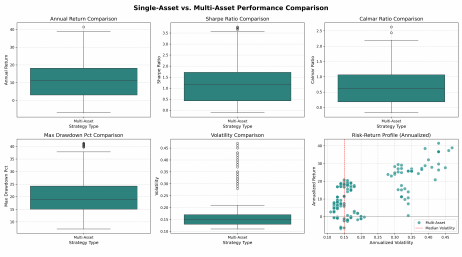
\includegraphics[width=4.80099in,height=2.66755in]{TongjiThesis-master/figures/media/image15.png}

\begin{quote}
\textbf{图4：}多资产策略在不同指标中的分布（箱线图与风险收益结构）

在低波动率高回报区间， 中位波动率红线更凸显了多资产配置的 稳健优势。

总体而言，多资产策略不仅实现了卓越的收益水平，同时在风
险控制和收益波动性方面也展现出稳健的性能。通过将统计数据
与可视化分析相结合，该策略为MAA提供了更丰富的协同信息和
更稳定的建模基础，成为其优异表现的关键要素。
\end{quote}

\emph{4.3.6. 任务类型与预训练融合组合的综合性能比较}

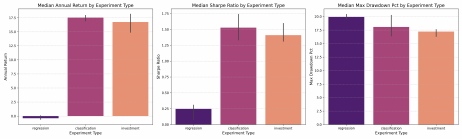
\includegraphics[width=4.80099in,height=1.44048in]{TongjiThesis-master/figures/media/image16.png}

\begin{quote}
\textbf{图s：}不同任务类型年化回报率中位数、夏普比率及最大回撤的比较

为深入分析各类任务与策略组合的综合表现，我们从两个维度
展开研究：一是回归、分类、投资等任务类型中风险收益指标的
中位数表现，二是不同预训练方法与融合机制组合后的平均夏普
比率分布。图\hyperref[bookmark52]{5}展示了各类任务指标中位数的对比结果。

该投资任务在收益生成与回撤控制两方面均表现出最优性能，
表明此类策略更擅长实现风险与收益的平衡。分类任务获得最高
夏普比率，凸显其在风险调整收益方面的潜力。尽管回归任务整
体表现稍逊，但仍保持正向中位数收益，展现出一定的稳健性。
图\hyperref[bookmark53]{6}进一步展示了不同预训练类型与融合机制组合的平均夏普比率
热图。
\end{quote}

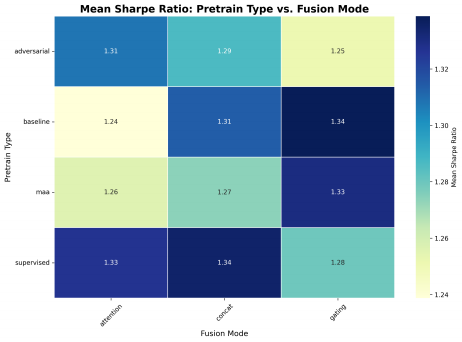
\includegraphics[width=4.80099in,height=3.55286in]{TongjiThesis-master/figures/media/image17.png}

\begin{quote}
\textbf{图6：}不同预训练类型与融合机制组合的平均夏普比率热图

MAA与门控机制的组合平均夏普比率高达1.33 ，显著优于其他
组合方案，充分验证了MAA在动态信息整合方面的优势。监督学
习与注意力/拼接机制的组合同样展现出优异的夏普指标，表明浅
层监督特征在特定融合机制中仍具有效性。对抗训练方法则表现
出更高的波动性，尤其在注意力机制下性能明显下降，这说明对
抗训练策略的融合兼容性仍需深入研究。

本节从任务类型和预训练融合结构两个维度，系统梳理了该模
型的综合性能。总体而言，MAA架构与门控融合机制的组合在多
数场景下表现稳定且优势显著，其中分类任务和投资任务最能充
分释放其潜力，这充分体现了该策略的强通用性和适应性。

\emph{4.3.7. 资产类别与资产多元化对策略绩效的影响分析}

在本节中，我们将从两个维度深入分析MAA策略中不同资产类
别的表现：一是各资产类别在年化收益率、夏普比率和最大回撤
等指标上的分布差异，二是不同资产组合规模对波动性的影响，
从而验证分散投资的效应。图\hyperref[bookmark54]{7}展示了能源、金属、化工和农业等
细分市场， 以及小型集团、大型集团和整体资产池（全集团）等
组合形式下，多个资产类别在三个关键指标上的箱线图分布。其
\protect\phantomsection\label{bookmark54}{}中化工资产类别展现出最优
\end{quote}

%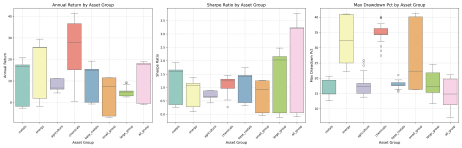
\includegraphics[width=4.80099in,height=1.52778in]{ TongjiThesis-master/figures/media/image18.png}

\begin{quote}
\textbf{图7：}不同资产类别在年化收益率、夏普比率和最大回撤方面的表现

该产品在年化收益率和夏普比率方面表现优异，但其最大回撤率
也相对较高，因此被归类为高风险、高回报型产品。该大型资产
组合展现出平衡收益与风险的能力，其夏普比率与最大回撤率均
呈现良好均衡状态，适合稳健投资。全组资产整体表现强劲，表
明广泛资产配置对MAA策略具有显著优势。农业和贱金属类资产
波动性较低，但整体收益能力普遍较弱。图\hyperref[bookmark55]{8}进一步揭示了``
资产 数量''与`` 年化波动率'' 的关系，清晰展现了分散化投资的风控
效果。资产数量较多的组合波动性更低，拟合曲线显示显著负相
关性。这一现象充分证明了资产分散配置的...
\end{quote}

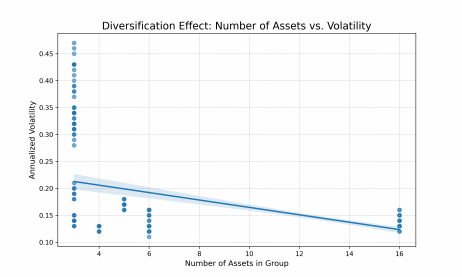
\includegraphics[width=4.80099in,height=2.88095in]{TongjiThesis-master/figures/media/image19.png}

\begin{quote}
\textbf{图8：}资产数量对年化波动率的影响（分散效应）

对冲系统性风险的对冲策略，这也是MAA在多资产环境中表现强
劲的根本原因之一。

不同资产类别的风险收益结构存在显著差异，这表明多资产模
型（MAA）在资产选择和结构学习方面具有适应性。同时，资产
分散化带来的波动抑制效应进一步凸显了多资产建模在量化投资 中的重要性
。总体而言，MAA策略有效利用资产异质性和多样
性，实现了收益与稳定性并重的投资目标。

\emph{4.4. MAA战略优势与特征分析}

\emph{4.4.1. 不同融合方法下MAA策略的性能}

本节评估了不同信息融合机制（\emph{注意力}、\emph{拼接}、 \emph{门控}）在
MAA预训练策略下对最终模型性能的影响。通过比较收益率、波
动率和风险调整收益率等关键指标，我们发现门控融合方法在多个关键维度上始终表现最佳，表明其与MAA策
\protect\phantomsection\label{bookmark56}{}略具有最强的协同融合效应。
\end{quote}

表\hyperref[bookmark56]{6}总结了三种融合方法的平均性能。
\textbf{表6：}不同融合方法下MAA策略的性能比较

采用门控融合技术的MAA策略展现出显著提升的收益生成能
力，平均回报率达到54.48\% ，明显优于注意力机制（50.98）和串
联策略（51.57）。此外， 门控融合在风险调整后表现更胜一筹，
不仅创下1.33的夏普比率和0.678的卡尔玛比率，更展现出卓越的
收益生成能力与风险管控能力。该策略年化回报率达12. 12\% ，在
众多融合方法中拔得头筹，堪称长期量化策略部署的理想选择。

\begin{quote}
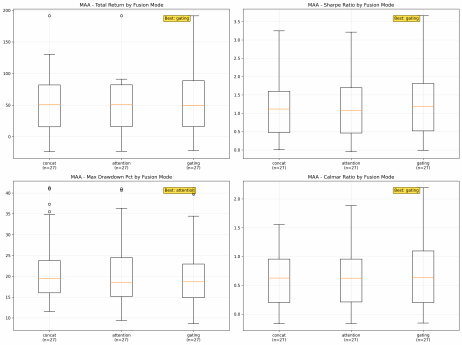
\includegraphics[width=4.80099in,height=3.58962in]{TongjiThesis-master/figures/media/image20.png}

\textbf{图9：}不同融合方法下MAA策略的性能分布（箱线图对比）

为直观展示不同融合机制下的绩效分布特征，
图\hyperref[bookmark57]{9}从分布层面
进一步验证了门控融合策略的稳健性。在收益分布方面， 门控模
式展现出略高的中位数收益和更强的尾部收益，表明其超额收益
能力更胜一筹。夏普比率分布整体更高且离散度更低，说明其风
险调整后收益的稳定性更强。在最大回撤方面，虽然注意力模式
的最小回撤略优，但门控模式的整体分布更为紧凑，使得极端风
险更易控制。最后，在卡尔玛比率中， 门控模式在中位数和上分
位数上均表现领先，展现出更优的回撤与收益平衡。

统计表与分布可视化均证实了门控融合机制与MAA策略之间存 在显著的协同优势。
门控机制能够动态调整各类特征子空间的重
要性，从而增强MAA在面对复杂异质特征输入时表现出的性能稳定性和风险适应
性。因此，我们建议在实际部署MAA框架时优先采用门控（Gat-
ing）作为融合机制。

\emph{4.4.2. 不同任务类型中MAA策略的性能分析}

为评估MAA策略的跨任务适应性，我们比较了其在三种任务类 型中的整体表现：
回归预测、分类预测和投资决策。统计结果见
\protect\phantomsection\label{bookmark58}{}表\hyperref[bookmark58]{7}。

\textbf{表7：}不同任务类型下MAA的性能比较
\end{quote}

\begin{quote}
如表所示 ，MAA 在分类任务中实现了最优的风险调整回报
（Sharpe和Calmar指标），在投资任务中则获得最高回报，充分证
明了其在不同目标函数下的灵活适应性。

为更直观地展示MAA策略的稳定性和卓越性能，我们绘制了各
\protect\phantomsection\label{bookmark59}{}类任务的分布情况，如图\hyperref[bookmark59]{10}所示。回收率分布（左图）
\end{quote}

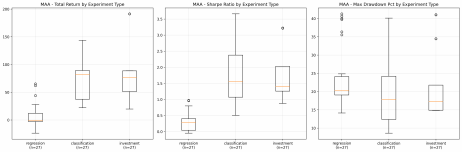
\includegraphics[width=4.80099in,height=1.57818in]{TongjiThesis-master/figures/media/image21.png}

\textbf{图10：}不同任务类型下MAA策略的性能分布（箱线图对比）
表明投资与分类任务均呈现高中位数回报率与更宽泛的上尾分布表明，多数实验呈现持续正向
回报，个别案例则获得异常高额回报。夏普比率（中间图表）显
示分类任务的夏普分布更为集中且向上偏斜，反映出风险调整后
回报的稳定性更高。最大回撤（右侧图表）揭示投资任务的最大
回撤分布相对紧凑，具有更低的最小值和中位数，证明其风险管
控能力更胜一筹。

\begin{quote}
综合表格与图表分析结果表明，MAA策略在分类任务中展现出
卓越的稳定性和抗风险能力， 同时在投资任务中实现了最高回报
目标。尽管回归任务因固有的高噪声和弱标签结构表现欠佳，但
仍保持正向回报，显示出一定的稳健性。

总体而言，MAA策略在多种任务类型中均表现优异，尤其在风
险调整回报（分类）和收益最大化（投资）方面形成互补优势，充
分验证了其作为通用金融特征建模解决方案的有效性与实用性。

\protect\phantomsection\label{bookmark60}{}\emph{4.4.3.
MAA与其他策略的总体绩效比较分析}
\end{quote}

为全面评估MAA策略相较于传统方法（包括监督学习和对抗性 强化学习）
的整体收益与风险表现，我们通过统计分析比较了若
干关键绩效指标：总回报率、年化回报率、最大回撤率、夏普比
率和卡尔玛比率。表\hyperref[bookmark60]{8}汇总了不同方法各指标的均值与中位数，并
展示了MAA策略相较其他方法的百分比提升幅度。

\begin{quote}
\textbf{表8：}MAA与其他策略的关键指标比较（均值/中位数/改善率）
\end{quote}

\begin{quote}
MAA策略展现出更稳健的收益稳定性：虽然其平均收益率与其 他策略相当
，但中位总回报率和年化收益率更高 ，且异常值更 少
，表明其在收益生成方面具有更强的持续性 。在风险控制方
面，MAA策略展现出均衡的风险管控能力：其最大回撤中位数略
低，表明其对回撤风险的控制水平与其他方法相当。在风险调整
后收益方面，MAA的绩效略逊一筹：其夏普比率和卡尔玛比率与
其他策略相近，但中位数略低，这可能与其收益波动特性有关。

总体而言，MAA策略在收益生成和稳健性方面均展现出显著优
势，尤其在中位数收益和回撤控制方面表现突出，这些特性对实
际投资部署至关重要 。尽管在某些风险调整比率上可能略显滞
后，但MAA策略提供了更为均衡的风险收益特征，使其特别适合
在复杂市场环境中稳定运行。

\emph{4.4.4. 多任务场景下MAA策略与其他预训练方法的性能对比}

为全面评估多任务注意力对齐（MAA）策略在金融预训练任务
中的表现，我们针对三种任务类型（回归、分类、投资决策）与
三种常见预训练方法（基线、监督、对抗）进行了对比分析，从
错误率、准确率和收益性三个维度进行评估。相关实验结果详见
表\hyperref[bookmark61]{9}至表\hyperref[bookmark62]{12}。

\textbf{表9：}回归任务均方误差（MSE）对比
\end{quote}


\begin{quote}
\textbf{表10：}分类任务的准确率对比
\end{quote}

{\def\LTcaptype{none} % do not increment counter
\begin{longtable}[]{@{}
  >{\raggedright\arraybackslash}p{(\linewidth - 6\tabcolsep) * \real{0.2144}}
  >{\raggedright\arraybackslash}p{(\linewidth - 6\tabcolsep) * \real{0.1834}}
  >{\raggedright\arraybackslash}p{(\linewidth - 6\tabcolsep) * \real{0.2348}}
  >{\raggedright\arraybackslash}p{(\linewidth - 6\tabcolsep) * \real{0.1989}}@{}}
\toprule\noalign{}
\endhead
\bottomrule\noalign{}
\endlastfoot
\begin{minipage}[t]{\linewidth}\raggedright
\begin{quote}
\textbf{预训练类型}
\end{quote}
\end{minipage} & \begin{minipage}[t]{\linewidth}\raggedright
\begin{quote}
\textbf{天} \textbf{青} \textbf{霉} \textbf{素}
\end{quote}
\end{minipage} & \begin{minipage}[t]{\linewidth}\raggedright
\begin{quote}
\textbf{Fu-Gating融合}
\end{quote}
\end{minipage} & \begin{minipage}[t]{\linewidth}\raggedright
\begin{quote}
\textbf{注意融合}
\end{quote}
\end{minipage} \\
\begin{minipage}[t]{\linewidth}\raggedright
\begin{quote}
基准
\end{quote}
\end{minipage} & \begin{minipage}[t]{\linewidth}\raggedright
\begin{quote}
0.6472
\end{quote}
\end{minipage} & \begin{minipage}[t]{\linewidth}\raggedright
\begin{quote}
0.6555
\end{quote}
\end{minipage} & \begin{minipage}[t]{\linewidth}\raggedright
\begin{quote}
0.6338
\end{quote}
\end{minipage} \\
\begin{minipage}[t]{\linewidth}\raggedright
\begin{quote}
监督
\end{quote}
\end{minipage} & \begin{minipage}[t]{\linewidth}\raggedright
\begin{quote}
\textbf{0.6558}
\end{quote}
\end{minipage} & \begin{minipage}[t]{\linewidth}\raggedright
\begin{quote}
0.6476
\end{quote}
\end{minipage} & \begin{minipage}[t]{\linewidth}\raggedright
\begin{quote}
\textbf{0.6543}
\end{quote}
\end{minipage} \\
\begin{minipage}[t]{\linewidth}\raggedright
\begin{quote}
对抗
\end{quote}
\end{minipage} & \begin{minipage}[t]{\linewidth}\raggedright
\begin{quote}
0.6457
\end{quote}
\end{minipage} & \begin{minipage}[t]{\linewidth}\raggedright
\begin{quote}
0.6357
\end{quote}
\end{minipage} & \begin{minipage}[t]{\linewidth}\raggedright
\begin{quote}
0.6535
\end{quote}
\end{minipage} \\
\begin{minipage}[t]{\linewidth}\raggedright
\begin{quote}
\textbf{最大认可度}
\end{quote}
\end{minipage} & \begin{minipage}[t]{\linewidth}\raggedright
\begin{quote}
0.6393
\end{quote}
\end{minipage} & \begin{minipage}[t]{\linewidth}\raggedright
\begin{quote}
\textbf{0.6542}
\end{quote}
\end{minipage} & \begin{minipage}[t]{\linewidth}\raggedright
\begin{quote}
0.6354
\end{quote}
\end{minipage} \\
\end{longtable}
}

\begin{quote}
\textbf{表11：}投资任务分类准确率对比
\end{quote}

\begin{quote}
此外，为了更直观地展示该策略在投资回测中的表现，图\hyperref[bookmark63]{11}展
示了MAA策略与其他方法在盈利能力和风险方面的对比图，相关
数值详见表\hyperref[bookmark62]{12}。

\textbf{表12：}后测表现（投资回报率、风险及夏普比率）对比
\end{quote}

\begin{quote}
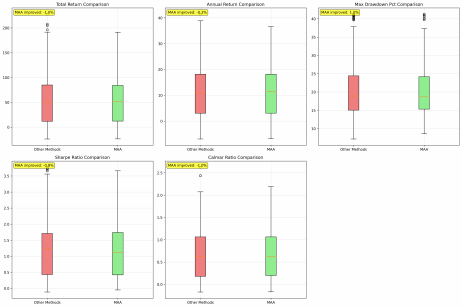
\includegraphics[width=4.80099in,height=3.18765in]{TongjiThesis-master/figures/media/image22.png}

\textbf{图11：}MAA策略与其他方法在多个指标上的回测比较

%\protect\phantomsection\label{bookmark64}{}最后，表\hyperref[bookmark64]{13}列出了不同资产类别中获得的最佳夏普比率，进一
%步凸显了MAA在``全资产类别''类别中的优势。

\textbf{表13：}各资产类别的最佳夏普比率
\end{quote}

\begin{quote}
尽管MAA在所有任务中可能无法实现绝对领先精度，但其在注
意力融合（Attention Fusion）下的多项关键指标（如夏普比率和卡
尔马比率）均表现出稳健性能。值得注意的是，其夏普比率最高 （3.771）。

在``全组资产''框架内，这凸显了MAA在复杂资产结构中卓越的
\protect\phantomsection\label{bookmark65}{}适应性和泛化能力。为进一步量化其稳健性与高端潜力
\end{quote}

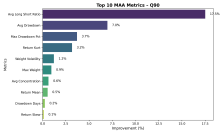
\includegraphics[width=2.30443in,height=1.38283in]{TongjiThesis-master/figures/media/image23.png}
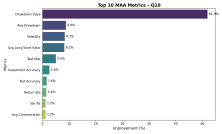
\includegraphics[width=2.30443in,height=1.38283in]{TongjiThesis-master/figures/media/image24.png}

\begin{quote}
\textbf{图12：}MAA在关键指标第10和第90百分位数上优于其他预训练策略

MAA策略，我们针对多个统计分位数进行了详细的前N指标改进
分析。具体而言，我们考察了MAA在所有评估指标上相对于其他
方法的第10百分位（Q10）和第90百分位（Q90）改进百分比。如 图
\hyperref[bookmark65]{12}所示 ，MAA 在Q10 水平 的 下行风 险指标上表现 出
显著 改 进------最明显的是\emph{回撤天数}减少了61.9\%
，同时在\emph{平均回撤}和\emph{波}
\emph{动率}方面也取得了显著提升，这反映了MAA即使在最坏情况下仍
具备卓越的风险控制能力。相反，在Q90水平上，MAA在投资组
合动态和资本效率方面也展现出明显优势，其中17.\emph{平均多空比率} 提升5\%
，同时\emph{最大回撤百分比}和\emph{收益率峰度}持续优化。这些数据
表明，MAA不仅在市场不利条件下表现稳健，即便在有利市场中
也能保持良好扩展性，充分验证了其在金融学习任务中兼具稳健
性与灵活性的优势。

除逐点比较外，我们还通过热图分析全面呈现了MAA策略在32
项关键指标和8个统计百分位数（最小值、第10百分位、第25百分
位、中位数、第75百分位、第90百分位、最大值、平均值）上的
相对改进百分比（详见图\hyperref[bookmark66]{13}）。该可视化图表清晰展示了MAA策
略在32项关键财务与行为指标及其对应8个统计百分位数（最小
值、第10百分位、第25百分位、中位数、第75百分位、Q90
、最大值、均值）。通过热图分析跨多种统计量
\end{quote}

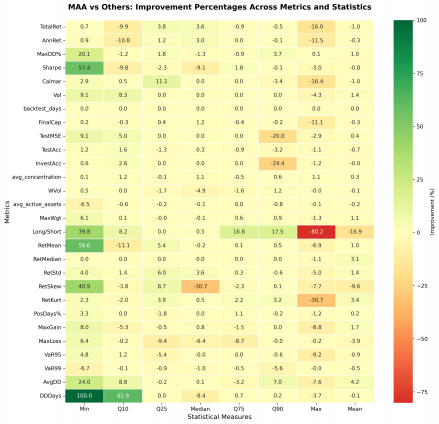
\includegraphics[width=4.56098in,height=4.41543in]{TongjiThesis-master/figures/media/image25.png}

\textbf{图13：}与其它预训练方法相比，32项指标和8个统计百分位数的MAA改
进百分比热图

通过计算量化指标（最小值、第10百分位数、中位数、第90百分
位数、最大值），可以明显看出MAA策略并非在所有指标或分位
数上都占据主导地位，而是根据所采用的统计量不同，在不同维
度上展现出相对优势。具体而言，当指标在较低分位数（如第10
百分位数或第25百分位数）进行排序分析时，MAA在风险相关维
度（如回撤天数、平均回撤值和波动率）上始终优于其他方法。
这表明在最坏情况或保守场景下，MAA具有稳健性优势。热力图
清晰地凸显了MAA在多个绩效维度上持续且显著的提升效果。

\begin{quote}
特别是在风险管理与资本保值方面，MAA的卓越表现尤为突出。 以``
回撤天数''（DDDays）指标为例，该指标在最低百分位数上
实现了100.0\%的显著提升，充分展现了MAA完全规避基准方法中
最长回撤周期的非凡能力。这种稳健表现延伸至第10百分位数（Q
10）达到61.9\%的提升幅度，并在多数分位区间持续保持显著优
势，有力印证了MAA在不利市场环境中的卓越抗风险能力。类似 地 ， 平 均 回
撤 率（AvgDD）（如 Q10 分 位 数 8.8\%） 和 波 动 率
（Vol）（如最低分位数9. 1\% 、Q10分位数8.3\%）等指标在其较低
分位区间也持续呈现正向改善，进一步验证了MAA在提升风险管
控与投资组合稳定性方面的优势。值得注意的是，夏普比率指标
在最低百分位数上同样实现57.4\%的显著提升，表明即使在市场环
境不利时，MAA仍具备创造更优风险调整后收益的强劲潜力。
\end{quote}

值得注意的是，这种模式表明MAA策略可能具备某种隐性对冲
能力。在较为保守的市场环境中，该策略相较于同类产品能实现
稳定收益或降低亏损。虽然在极端高值区间（如某些指标的Q90或
Max）可能无法达到最佳表现，但其在低值区间保持稳健表现的能
力，凸显了其在风险规避型投资组合管理或市场波动条件下的实
用价值。此外，MAA在战术资产配置和收益分布特征等关键指标 上展现出显著提升
。例如 ，平均多空比率（Long/Short）在Q75
（16.8\%）和Q90（17.5\%）区间呈现正向改善，表明在常规至有利 市场条件下
，该策略能更精准地表达方向性判断并优化风险敞 口 。类似地 ，
收益偏度（RetSkew）在其最低百分位数处提升 40.9\%
，显示出更优的收益左尾分布特征。收益均值（RetMean）
在最低百分位数处也实现了58.6\%的显著提升。这些收益综合表
明，MAA具备优化整体回报结构并有效管理风险敞口的能力。

总体而言，MAA显示出非均匀但战略分布的改进，表明其在特
定市场压力条件下适在所有场景中，虽然整体趋势有力印证了MAA的优异表现，但通
过热力图的细致分析，我们仍能发现需要进一步优化和研究的具
体领域。某些指标（如年化收益率AnnRet ，最大值时为-11.5\%； 测 试 MSE
，Q75 时 为 -20.0\%； 投 资 精 准 度 InvestAcc ，Q90 时
为-24.4\%）在较高分位数区间呈现局部负向改善。这些现象并非
必然存在根本缺陷，而是暗示了过度优化的可能性，或是MAA在
极端有利条件下对特定市场环境的过度敏感------这种情况下，其
自适应定位策略可能导致偏离基准值的幅度更大。 同样，尽管夏
普比率显示出显著的最低改善，但在其他多个分位数区间却呈现
负向改善，这表明虽然MAA在最坏情况下能实现高风险调整回
报，但其在此方面的平均或典型表现可能需要进一步优化。这些
研究发现凸显了在真实交易系统中校准MAA部署的重要性，既要
确保其效益最大化，又需考量其对极端正向场景的敏感性。相关
成果为未来研究指明方向，推动MAA动态适应机制的开发，从而
进一步巩固其稳健的性能表现。

\begin{quote}
\emph{4.4.5. 最高总收益配置下MAA策略的性能分析}
\end{quote}

为了充分展示MAA主动回收的能力，我们选择了在所有实验中
产生最高总回报的配置：\emph{多化学品串联\ul{MAA}} 。该
配置以三种化学资产（聚氯乙烯、聚丙烯、聚对苯二甲酸乙二醇酯）作为建模基
础，通过串联融合方法在MAA预训练框架上构建。在回测期间，
该配置表现出卓越的资本增长，使其在所有实验中脱颖而出，成为表现最出色的配置之一。

在此配置下 ，MAA策略在863个交易日 中成功将初始资本从
2,000,000提升至3,235,581.20 ，累计回报率达61.78\% ，年化回报率 为15.08\%
。尽管该策略伴随一定波动性（最大回撤达35.52\%），
但其0.969的夏普比率表明风险控制水平保持合理。

\begin{quote}
应性更强，而非普遍优于其他方案。

在追求高回报的同时。

\textbf{表14：}MAA策略的关键绩效指标 \emph{\ul{多化学物质}串联}构型

\textbf{指标} \textbf{值} \textbf{描述}
\end{quote}


\begin{quote}
图\hyperref[bookmark67]{14}展示了该策略的整体收益曲线（左）
与收益分布直方图 （右） 。左图清晰显示在中后期阶段实现了显著的资本增长，
同
\protect\phantomsection\label{bookmark67}{}时整体控制性回撤，展现出稳健的稳定性。收益分布直方图显示
\end{quote}

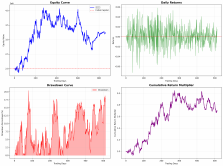
\includegraphics[width=2.30431in,height=1.72482in]{TongjiThesis-master/figures/media/image26.png}
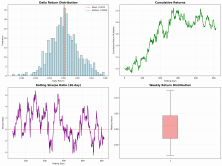
\includegraphics[width=2.30431in,height=1.72482in]{TongjiThesis-master/figures/media/image27.png}

\begin{quote}
\textbf{图14：}化工资产组MAA策略回测收益率曲线及收益率分布

贡献度分布图显示轻微正偏态，正收益占主导地位，表明存在明
显的盈利偏好和有效尾部风险

控制极端负回报事件有限的分布。该分布-该公司的特征进一步证明，即便在高回报环境中，其夏普比率仍
\protect\phantomsection\label{bookmark68}{}保持稳健。
\end{quote}

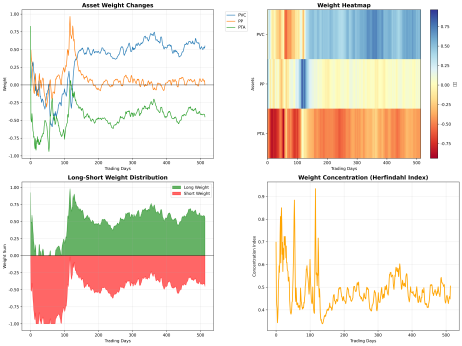
\includegraphics[width=4.80099in,height=3.5959in]{TongjiThesis-master/figures/media/image28.png}

\begin{quote}
\textbf{图15：}化学品资产组MAA策略动态资产配置权重

此外，图\hyperref[bookmark68]{15}展示了该策略在运行期间的动态资产配置权重。该策
略在三种化工资产中实现了稳定而灵活的仓位调整，凸显了MAA框
架在学习资产间结构特征方面的强大能力。

具体而言，PTA的平均权重为-0.4471 ，表明其持续处于空头头
寸，这表明该策略准确识别了其下行趋势。聚氯乙烯的平均权重 为0.3507
，作为主要的多头资产，持续贡献正回报。PP的权重波动最小，平均约为0.0962
，扮演着辅助多头的角色。

综上所述，该配置下的MAA策略在有效管理风险的同时实现了 显著的回报增长。

通过灵活的仓位调度和高效的资产结构学习，这一能力充分展示
了MAA在多资产量化建模中的高回报潜力和实际价值。

\textbf{5. 结论与未来工作}

本研究通过多类金融建模场景，系统评估了多智能体对抗策略
（MAA），涵盖不同资产类别、融合机制、实验类型及预训练方
法。基于大量回测数据的全面分析表明，MAA在复杂市场环境中展
现出卓越性能，尤其在风险管控与收益生成方面表现突出。

实验结果充分展现了MAA框架的多项核心优势。在多项性能指
标测试中，MAA不仅持续保持强劲回报表现，更显著降低了下行
风险------其最大回撤率的改善和风险调整后比率的优化就是有力
证明。当MAA与Gating融合机制结合使用时，这种稳健性得到进
一步强化。该机制通过动态加权多源特征，实现了信息整合的灵
活性与抗风险能力的双重提升。这种协同效应对于提升MAA在非
平稳市场条件下的性能稳定性与适应性至关重要。
\end{quote}

此外，我们对不同任务类型的探索揭示了MAA的卓越灵活性。
虽然分类任务受益于最优风险调整回报（夏普比率和卡尔玛比 率）
，但投资任务实现了最高的整体回报。这种双重优势验证了
MAA作为多功能金融特征建模解决方案的有效性，能够根据具体
投资目标调整其目标，优先考虑风险控制或回报最大化。对\emph{资产}
\emph{分散性}的分析也证实，MAA能有效利用资产异质性，分散化投资
组合始终表现出更低的波动性。这种整合互补性资产信息的内在
能力，是MAA在不同市场领域保持稳健稳定表现的根本所在。

\begin{quote}
尽管已证实其优势，未来仍存在若干研究与开发方向。首先，
虽然MAA表现出稳健性能，但需进一步探究其超参数优化方法。

首先，通过优化参数设置和网络架构，可以释放更大的潜力，尤
其能针对特定市场环境或资产类别量身定制交易策略。其次，整
合宏观经济指标与替代数据源（如新闻舆情、卫星影像等），能
提供更丰富的背景信息，从而提升MAA的预测精度和自适应能
力。第三，深入解析MAA决策机制的可解释性------特别是其多智
能体系统与对抗组件如何协同生成交易信号------对于增强从业者
信任度和理解度至关重要。最后，将MAA框架拓展至高频交易策
略或衍生品市场，这既是极具挑战性的课题，也要求实时数据处
理与执行能力实现突破性提升。

综上所述，MAA策略作为多资产量化投资的框架，兼具强大功
能与高度灵活性。其在复杂非平稳金融市场中展现的卓越稳定性
与风险管控能力，为自动化交易与投资组合管理领域的未来创新
奠定了坚实基础。我们相信，基于这些基础的持续研究将进一步
巩固其作为量化金融领域领先方法论的地位。
\end{quote}

\section{3.5小结}\label{ux5c0fux7ed3}

\section{第 4 章
基于孪生对抗机制的波浪预测问题}

\section{4.1 引言}

\begin{quote}
金融市场价格通常呈现出分形和周期性的波动模式\hl{{[}{]}}，然而，传统波浪预测方法如ARIMA或GARCH往往难以应对高频且非平稳的市场环境。因此，Elliott波浪理论作为一种强调市场参与者心理驱动因素以及价格变动周期性波浪特征的结构分析框架，自20世纪中期出现以来，已在股票、期货和加密货币等市场得到广泛应用。但Elliott波浪理论在波浪划分上，严重依赖人类主观判断，边界定义模糊，难以实现自动化和标准化识别。

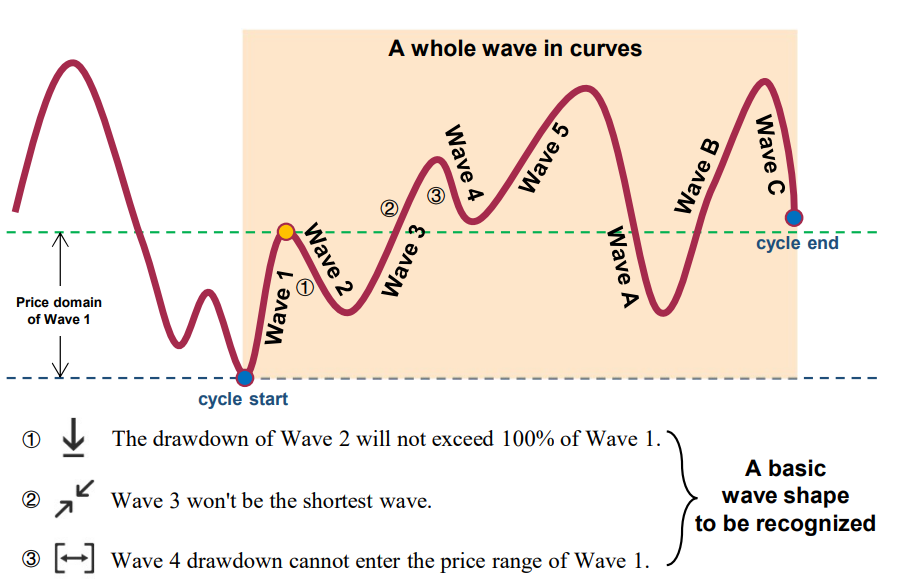
\includegraphics[width=4.26597in,height=2.76389in]{TongjiThesis-master/figures/media/image29.png}

图：Elliott波浪理论

为解决具有不同特征的波浪识别问题，本文提出了一种结合多智能体群组交叉对抗机制的波浪预测方法，采用多智能体群组交叉（MGCA）对抗框架，通过联合训练多个智能体，并利用多尺度时间卷积核自注意力机制，自主识别和区分各类分形波结构。同时，针对多智能体对抗过程中异质性导致的对抗崩溃问题，我们提出了一种基于蒸馏学习的反向知识蒸馏算法。多智能体系统具备跨尺度建模、多任务学习和结构感知等能力，为识别金融时间序列中复杂的层级运动模式提供新颖的方法，并为将传统技术分析与现代深度学习技术相结合开辟了新途径。
\end{quote}

\section{4.2 研究背景}

\begin{quote}
4.2.1 波浪理论与市场预测

Elliott波浪理论由艾略特于20世纪提出，是一种分析市场行为的结构化方法。该理论的核心观点是，市场波浪通常先以五浪推进结构（推动浪）展开，随后是三浪调整（调整浪），且这类模式会在不同时间尺度上递归嵌套，从而呈现出分形特征\hl{{[}{]}}。

在实践中，Elliott波浪理论已被广泛应用于识别波浪的延续与反转、预测价格走势以及划定风险区域\hl{{[}{]}}。然而，由于金融市场固有的高频噪声和结构模糊性，仅有部分波浪片段具有实际预测意义和交易价值。因此，在现代复杂金融市场中，尤其是在高频数据环境或多资产交互系统中，Elliott波浪理论的独立结构分析面临明显瓶颈。迫切需要将其与数据驱动方法相结合，以提升波浪结构识别的自动化、客观性和适应性。

4.2.2 VA/CD分形的定义

交叉导数（CD）分形是一种整合了波信号与反转信号的结构化分割方法，旨在为分形波浪理论提供可量化、可重复的建模方案。该方法通过检测不同周期的移动平均线之间的交叉点来实现分割。具体而言，若交叉段的端点价格与起点价格保持同向且变动幅度显著，该线段将被标记为有效波浪；反之，若价格在该线段内震荡且无明确方向性或连续性，则标记为无效波浪。这种分类方式既继承了波浪理论中推动浪与调整浪的核心概念，又通过信号驱动的分形建模实现了波浪结构的自动化识别与分类。

交叉导数（CD）分形通过对市场价格运动的分割，能够清晰地划分出有价值的波浪模式，这些波浪模式通常具有明显的方向性和连续性，代表着价格的趋势发展。而相对的无效波浪则可能是市场的震荡区域，波动幅度较小，缺乏明确的趋势指引。通过这种方法，市场中潜在的波动模式能够被更加精确地识别，为波浪理论的实际应用提供了一个坚实的基础。

顶点邻接（VA）分形源自市场轮廓理论中的价值区域概念，聚焦于价格在高成交量区域附近随时间演变的分形行为。该方法为分形波浪分割引入了基于密度的视角，丰富了系统对价格结构性特征的识别能力。VA分形模型通过考虑市场参与者的交易行为，尤其是高成交量区域的影响，进一步优化了价格波动的识别能力。在这些区域内，价格的波动更具有结构性和规律性，且通常能反映出市场对特定价格水平的认同或反应。因此，VA分形为波浪模式的识别提供了额外的市场深度信息，使得模型在波浪结构的分割上更加精确。

在定义CD和VA分形规则后，将这些方法应用于期货市场的原始K线序列，构建出嵌入分形结构感知的监督学习数据集。通过这种方式，模型能够自动地识别和分类不同的波浪模式，并基于历史数据学习市场的波动规律，从而在未来的市场预测中提供更可靠的参考。结合CD和VA分形的技术，使得波浪理论的实际应用不再依赖手工分析和复杂的理论推导，而是通过自动化的方式进行高效、准确的市场趋势预测和风险评估。
\end{quote}

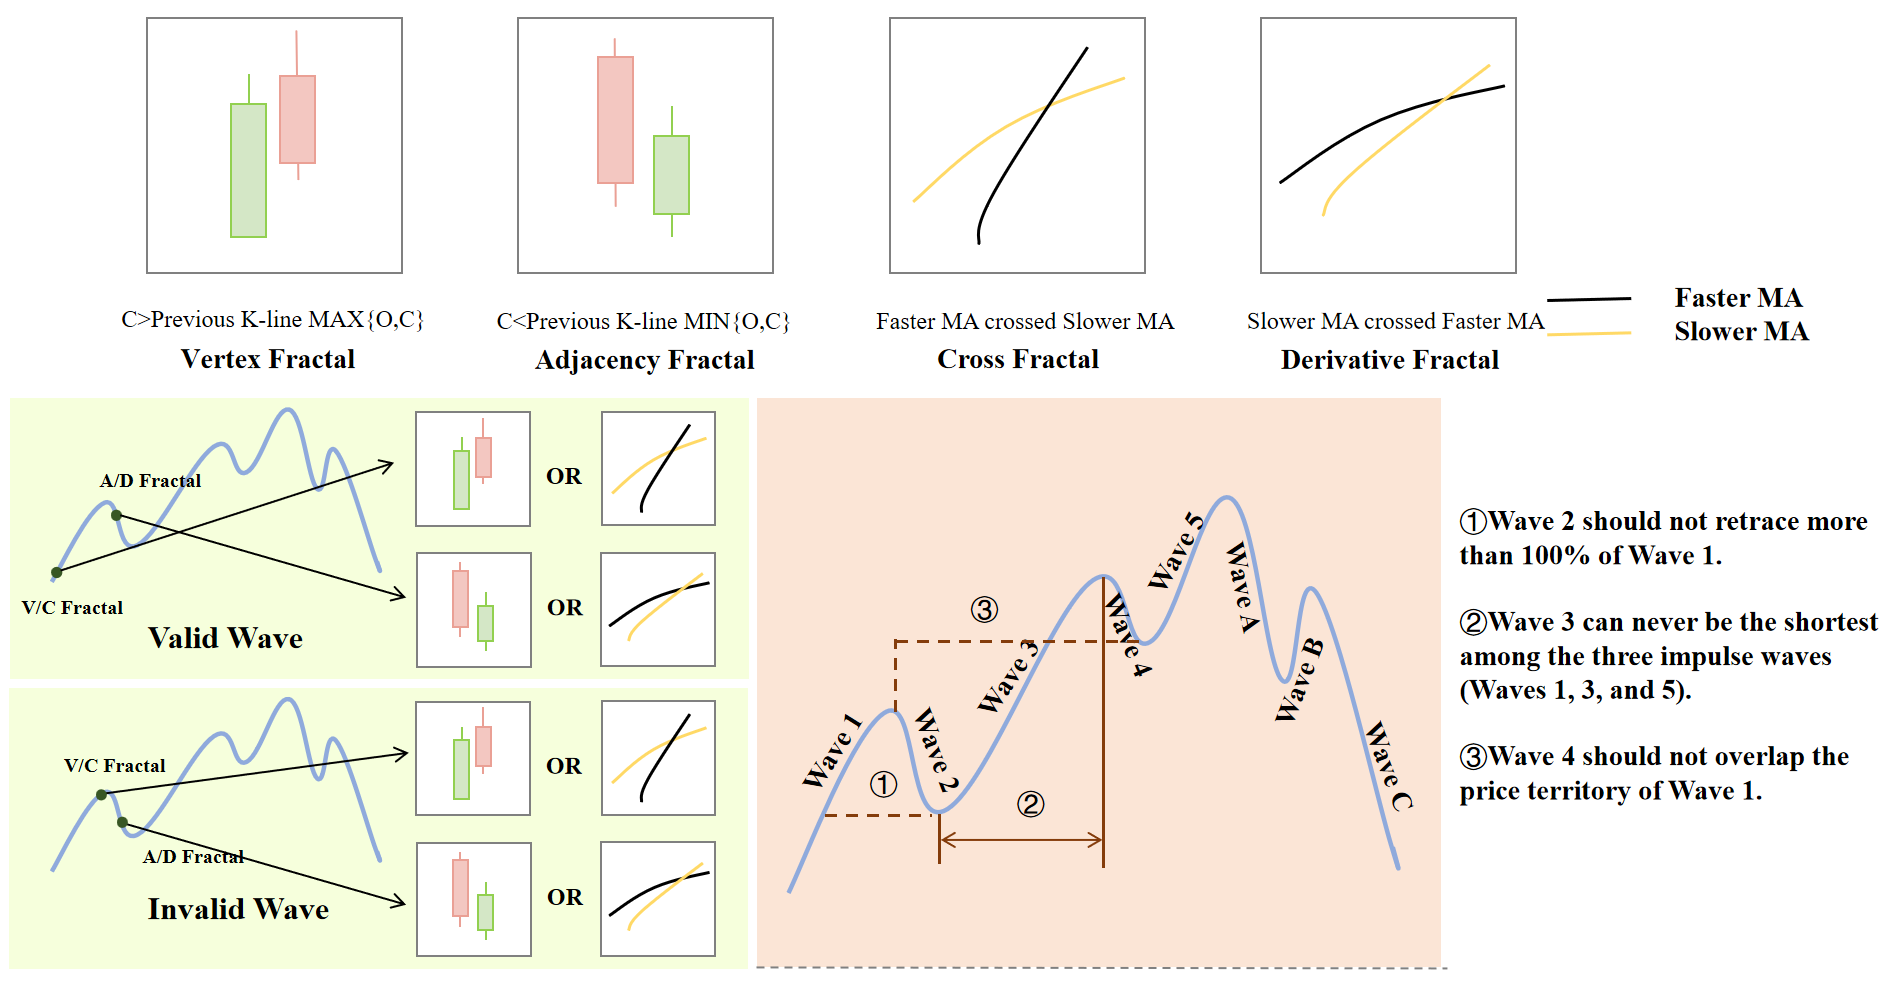
\includegraphics[width=5.40833in,height=3.00208in]{TongjiThesis-master/figures/media/image30.png}

\begin{quote}
图：CDVA分型分割有效波浪任务

4.2.3 金融预测中的深度学习

深度学习在金融时间序列预测中展现出显著优势，已成为智能量化交易和风险管理系统的关键支撑技术\hl{{[}{]}}。在各类网络架构中，长短期记忆（LSTM）网络\hl{{[}{]}}和
Transformer
模型\hl{{[}{]}}因具备捕捉长期时间依赖关系的能力，被广泛应用于趋势检测、波动率预测和信号生成任务。生成对抗网络（GANs）\hl{{[}{]}}在金融领域的应用也日益兴起，尤其适用于合成数据生成、场景模拟和风险建模等场景。

然而，在非平稳条件或结构突变下，这些模型的性能往往会下降。此外，深度学习模型对超参数设置和输入数据分布较为敏感，导致模型调优成本高、鲁棒性有限。同时，其缺乏可解释性的特点，也给需要透明度和问责制的风险敏感场景带来了挑战。
\end{quote}

\section{4.3 算法机制}

\begin{quote}
4.3.1 多组交叉对抗框架

MGCA
框架包含两个核心组件：多智能体生成器和跨智能体判别器。每个生成器采用不同的骨干网络架构（如GRU、LSTM、Transformer）处理输入序列，并输出一组分类和回归目标，包括波浪模式、趋势持续时间和结构标签。智能体判别器在对抗训练过程中评估每个生成器输出的真实性和一致性，同时提升智能体间的特征区分能力。

输入数据包括开盘价、最高价、最低价、收盘价（OHLC）等价格数据，并辅以趋势敏感指标（如
5 日指数移动平均线 / 120
日指数移动平均线）。输出部分包含多个任务特定的输出头，包括三个波浪分类头（CD1、CD2、CD3）、一个波动率关注标签（VA）以及一个用于趋势持续时间估计的回归头。

创建多个生成器组与判别器组，每个生成器组包含多个不同架构的生成器模型（如MAA、GRU、LSTM），每个判别器组包含多个不同架构的判别器模型（如MLP、LSTM、Transformer），对每对不同组的生成器和判别器进行训练，利用打分器（验证集MSE或CE）来评估生成器和判别器的表现。

其中，生成器的损失定义为：

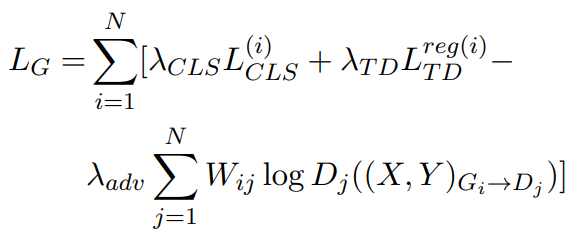
\includegraphics[width=2.81736in,height=1.14653in]{TongjiThesis-master/figures/media/image31.png}

判别器的损失定义为：

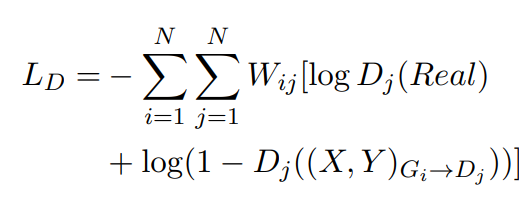
\includegraphics[width=2.80208in,height=1.06319in]{TongjiThesis-master/figures/media/image32.png}

4.3.2 结构引导的投资组合优化

为将MGCA的结构化预测结果转化为可执行的投资决策，本文基于波浪分类和趋势持续时间估计的双任务输出，设计了投资组合配置策略。具体来说，基于MGCA框架的预测输出，包括波浪分类（CD1、CD2、CD3）和趋势持续时间估计（回归头的输出），构建一个动态的投资组合配置系统。该策略通过确定有效波浪的方向和持续时间，从而指导投资决策，进而优化投资组合的风险收益比。

4.3.3 权重构建

在投资组合优化过程中，我们基于模型的信心水平来构建每个资产的权重。设定每个资产在某一时刻形成有效波浪的信心得分为
%\hl{}，以及预期的趋势持续时间得分为
%\hl{}。综合信心得分可以通过以下公式计算：

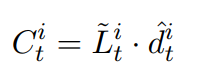
\includegraphics[width=1.0625in,height=0.41667in]{TongjiThesis-master/figures/media/image33.png}

随后，资产的投资权重通过对所有资产的综合信心得分进行标准化计算：

%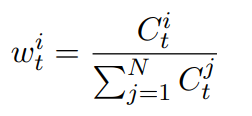
\includegraphics[width=1.28125in,height=0.58958in]{TongjiThesis-master/figures/media/image34.png}

这种权重构建方式能够动态调整每个资产在投资组合中的比例，确保投资组合的优化和风险控制。

4.3.4 反向知识蒸馏

反向知识蒸馏以两个预训练模型D1和D2为输入，通过评分器得到他们对应的性能分数S1和S2。该算法以阈值Phi作为终止条件，当两个模型的性能差距满足\textbar S1-S2\textbar\textgreater Phi时，进入循环式对抗学习阶段。

%在循环过程中，系统通过条件判断逻辑评估当前模型间的性能差距：若S1\textgreater S2，则由模型D2引导模型D1，实现D1反向学习；若S2\textgreater S1，则由模型D1引导模型D2，实现D2的反向学习。通过持续的反向引导与参数更新，两个模型的性能差距会逐步缩小。当\textbar S1-S2\textbar\textless Phi时，循环终止，系统输出经过反向学习优化后的更新模型D1和D2，完成反向知识蒸馏的全流程。反向知识蒸馏的算法逻辑如\hl{图}所示。

（1）群组交叉对抗

我们进行两对GAN的对称性训练，每个生成器和判别器在其所属的群组内独立训练。每次训练后，生成器和判别器通过计算损失值，根据表现选择最优模型。最优的生成器和判别器将被用来引导落后模型进行学习。

在组内对抗训练后，来自不同组的生成器和判别器将进行对抗训练。最优生成器和最优判别器作为教师模型，用于后续训练。

（2）赛马场训练

学习生成市场序列数据，并与真实数据按比例混合，使用混合数据训练新的学生生成器和判别器，如果学生模型性能优于现有模型，替换最差的模型位置。

（3）双向蒸馏

双向蒸馏机制的核心目标是通过教师-学生模型的训练方式，利用最优模型指导表现较差的模型。具体来说，我们使用最优生成器和判别器作为教师模型，引导学生模型学习其输出。通过打分器评估每个生成器组和判别器组，群组内的生成器和判别器会进行一对一的GAN训练，通过最差模型拟合最优模型的输出，不断在群组内循环进行评分学习。

双向蒸馏的算法逻辑如图所示

（4）Twin孪生对抗检测

Twin孪生对抗检测是通过统计每个生成器与最优生成器之间的MSE或CE超阈值次数，来判断模型是否达到预期性能。当生成器与最优生成器之间损失超出预设的阈值次数，则判断该模型表现不佳，进行模型替换。

4.3.2 基线模型

基于MGCA的分配策略与两种常见基线进行了比较：
\end{quote}

\begin{enumerate}
\def\labelenumi{\arabic{enumi}.}
\item
  等权重（EW）
\item
  均值-方差优化（MVO）
\end{enumerate}

\section{4.4实验结果分析}

\begin{quote}
为验证基于 VA/CD
分形模式的趋势识别方法及多智能体组交叉对抗（MGCA）架构的有效性，本研究选取中国市场
15
种主要商品期货作为研究对象，涵盖多个行业板块，具体包括：铜、玉米、精对苯二甲酸（PTA）、聚氯乙烯（PVC）、螺纹钢、豆粕、白糖、一号大豆、豆油、铝、锌、橡胶、棕榈油、棉花、黄金。

所有数据均为日度数据，包含开盘价、最高价、最低价、收盘价等基本字段。预处理阶段中，首先剔除节假日和非交易日数据，对缺失值采用前向填充法补充，并通过滑动窗口进行平滑处理，以确保时间序列的连续性和可计算性。

4.4.1整体性能比较

表全面比较了所有模型
\end{quote}

\section{4.5小结}

\section{第 5 章
基于群组交叉对抗的投资组合管理问题}

\section{5.1 引言}

\begin{quote}
在金融市场建模与资产配置领域，时间序列预测（TSF）面临两大核心挑战。首先，金融信号具有多尺度和高度异质性的动态特征，短期波动、中期结构与长期趋势往往共存。传统单一结构模型难以同时捕捉这些时间维度的信息。其次，主流预测模型通常采用误差最小化指标（如
MSE 、RMSE 或 MAPE）进行评估，但这些指标未能充分反映
预测信号在现实投资环境中的可交易性或经济价值（多明戈斯，2012；彭与德莫拉埃斯·索萨，2024）。正如
Xu
等人（2025）所指出的，此类指标往往忽视了信号质量维度，例如稳定性、方向准确性及边际效用等对投资组合决策的影响。这些局限性促使金融
TSF
界重新审视模型架构与目标函数设计，推动了更稳健且经济基础更扎实的预测框架发展。

为应对上述挑战，我们提出了一种新型多智能体对抗性时间序列预测框架（MAA-
TSF）。该框架整合了三种主流时间序列生成器：门控循环单元（GRU）、长短期记忆网络（LSTM）和基于Transformer的架构，分别擅长捕捉短期、中期和长期动态。每个生成器都与专用判别器配对，形成对抗性结构，使各智能体能够协同优化。这种架构设计使模型能更精准捕捉非线性和多频段模式，在结构波动和情绪驱动的市场环境中展现出更强的鲁棒性和泛化能力。

与传统方法仅关注最小化统计误差不同，MAA- TSF
引入了一个新颖且经济合理的优化目标函数。具体而言，我们通过将信号强度（反映交易性）和预测精度（体现方向准确性）这两个关键指标作为权重因子，纳入损失函数中。这种多维损失函数可抑制模型对低质量信号的过拟合，并引导模型生成的预测不仅具有统计学可靠性，同时具备经济可操作性及时间稳定性。

在策略层面，我们进一步开发了一种基于信号质量的动态因子配置机制。该机制以预测信号强度作为因子配置的筛选标准，并通过预测精度动态调整资产权重。相较于传统的静态因子模型或规则型再平衡方法，这种机制展现出更强的市场响应能力与超额收益生成潜力，从而具备更高的实际应用价值和跨市场可移植性。

总之，我们通过三个关键层面的创新构建了一个闭环预测-评估-执行系统：1)模型架构
，利用一种新颖的多智能体对抗学习方法来捕捉复杂的交互式市场动态；2)最优目标设计
，采用一种信号质量加权损失函数，优先考虑预测信号的经济意义和可靠性；3)
投资组合构建 ，使动态再平衡策略能够直接由框架的实时预测输出驱动。MAA-
TSF
框架不仅提升了对复杂时间结构的建模能力，更推动了金融预测领域的范式转变------从关注统计显著性转向重视经济可行性
。这为资产定价、策略制定和实时交易执行奠定了更实用的操作基础。

本章结构安排如下：第2节系统梳理相关文献；第3节阐述所建模型及实验方案；第4节展示预测结果；第5节评估投资组合策略的回测表现；第6节总结全文，重点阐述核心发现与未来研究方向。
\end{quote}

\section{5.2 研究背景}

\subsubsection{5.2.1
时间序列模型预测}

\begin{quote}
在时间序列预测领域，深度学习方法因其强大的非线性和非平稳结构建模能力而迅速受到关注。这些方法已被广泛应用于增强文本分析的传统方法（克劳斯和费尔里格尔，2017）、价格预测（费舍尔和克劳斯，2018），以及提升波动率估计和风险预警系统的稳健性与前瞻性性能（西里尼亚诺和康特，2021）。在金融应用领域，早期研究主要采用循环神经网络（RNN）及其变体，如长短期记忆网络（LSTM）（霍赫赖特和施密德胡贝尔，1997；金等人，2020）和门控循环单元（GRU；赵等人，2014），这些模型已被广泛应用于股价动态分析、波动率预测和因子收益建模（费舍尔和克劳斯，2018）。这些架构通过引入门控机制来缓解梯度消失问题，有效捕捉金融时间序列中的动态依赖关系。随着对建模长期依赖关系需求的增加，Transformer架构已成为金融领域极具前景的替代方案。

基于自注意力机制和高并行性的优势（Zhou 等，2021； Wu
等，2021），金融预测模型展现出更强的灵活性和稳定性，能有效捕捉不同市场环境下的动态变化。Transformer架构的改进版本------如Informer（Zhou
等，2021）和Autoformer（Wu
等，2021）------在长期预测中表现尤为突出，特别适合处理具有显著周期性和趋势特征的金融数据。与此同时，研究者们还通过结构优化来提升传统模型的复杂性，例如将多尺度建模融入
LSTM 框架： MLCA - LSTM 技术支持跨时间窗口的输入重要性加权建模（Teng
等，2022），而 LSTM - MLP 则减少了对显式波动率估计的依赖（Vinje
，2025）。Wang（2023）更是在Transformer编码器中整合了双向长短期记忆网络（BiLSTM）与时序卷积网络（TCNs），实现了局部特征与全局特征的协同建模。

然而，单一架构的预测模型在面对金融市场固有的异质性和剧烈波动时，往往表现出显著的不稳定性。这些模型难以有效适应高波动环境、结构性制度变迁或频繁的政策冲击（Gu
等，2020）。为提升模型在多样化金融场景下的稳健性和适应性，近期研究开始探索集成学习和生成对抗网络（GANs）（Zhou
等，2021； Krauss
等，2017）。集成方法通过聚合多个模型增强泛化能力，而GANs则能更有效地建模复杂分布和尾部风险。部分研究提出了结合卷积神经网络（CNNs）与Transformer及
LSTM
的混合深度学习框架，通过统一架构同时捕捉局部时间模式和长程依赖关系（Phyo
等，2021）。针对金融时间序列特征的模型创新日益普及（Wiese
等，2020）。基于这一趋势，Vuleti`c等（2025年）提出了一种专为金融预测设计的生成对抗网络（GAN）模型，该模型创新性地引入了经济学驱动的损失函数，使生成器能够输出条件概率分布而非简单的点预测。这种创新方法能更精准地刻画收益分布的不对称性与尾部特征。通过综合考量信号强度稳定性与预测区间不确定性，该模型在夏普比率等关键指标上实现显著提升，展现出在资产定价、风险管理及动态资产配置等领域的广阔应用前景（Vuleti`c
和 Cont ，2025）。
\end{quote}

\subsubsection{5.2.2
模型评价函数}

\begin{quote}
传统回归与分类任务通常采用交叉熵损失、均方误差（MSE）、均方根误差（RMSE）、平均绝对百分比误差（MAPE）和平均百分比误差（MPE）等标准指标（Si
等，2025）。虽然这些指标能有效衡量统计准确性，但往往侧重于样本内拟合，导致模型捕捉噪声而非有效结构特征，从而影响泛化性能（Domingos
，2012）。例如在财务预测中，模型可能过度拟合无关波动，对现实决策的实际价值有限（Peng
and de Moraes Souza，2024）。

为解决这些局限性，近期研究已转向评估预测信号的质量而非单纯关注其误差。部分文献提出了稳定性感知损失函数，通过惩罚信号过度波动来增强滚动预测的一致性（Jiang等，2023）。然而这类方法往往仅关注稳定性，而未考虑信号强度（如交易保证金）和方向准确性。一种更全面的视角逐渐形成，将经济表现、风险承受能力和趋势可操作性纳入模型评估框架，这在金融时间序列领域尤为重要------传统误差指标常与实际投资结果存在偏差。例如，
Moody
等（1998）率先将夏普比率作为强化学习的目标函数，实现了模型训练过程中对风险收益权衡的内生优化。这种基于经济原理的方法后来通过引入M
²
等绩效指标得以扩展。Sortino比率用于捕捉不同风险暴露水平下的风险调整后收益差异（MoralesArias
等，2013）。

此外，多目标优化方法的引入使模型能够同时考量收益、波动性和最大回撤，从而在稳健性与盈利能力之间建立动态平衡（Sahu
，2023）。这增强了模型在极端市场环境或不可预见风险下的抗风险能力。与此同时，为评估预测的可交易性与趋势一致性，研究者引入了动态相似性（DS）等结构化指标。这些指标通过方向性和转折点等维度，衡量预测序列与实际市场趋势的吻合程度，有效解决了预测结果虽数值精确却缺乏战略参考价值的局限性（Heng-Li
，2015）。
\end{quote}

\subsubsection{5.2.3
投资组合再平衡机制}

\begin{quote}
为了应对上述挑战，引入多智能体对抗学习具有明确的经济学和工程学动机。
从市场微观结构的角度来看，金融市场本身就是由持有不同预期、使用不同信息处理机制的异质代理人（Heterogeneous
Agents）博弈形成的。MAA-TSF 框架通过集成 GRU、LSTM 和 Transformer
等异构生成器，模拟了不同时间尺度偏好的市场参与者 。
而对抗学习（Adversarial
Learning）引入的判别器，则充当了``市场筛选机制''。通过生成器与判别器之间的博弈，模型被迫生成更符合真实市场分布特性的序列，从而提高了对尾部风险和非线性模式的捕捉能力
。这种多智能体的协同优化不仅仅是集成学习的堆叠，更是一种通过对抗博弈实现稳健性提升的动态过程。

金融市场可预测性一直是学术研究的核心议题。尽管有效市场假说（EMH）认为资产价格已充分反映所有可用信息，从而排除了持续预测的可能性（Fama
，2014），但越来越多的实证证据开始挑战这一观点。诸如价格反转现象------即此前表现不佳的股票未来可能获得超额回报------揭示了投资者过度反应等行为偏差（De
Bondt等，1985）。 Lo 和
MacKinlay（1988）通过方差比检验否定了随机游走假说，进一步证实价格动态中存在可预测成分。此外，持续存在的异常现象，包括一月效应、规模效应和动量效应，仍在不断动摇
EMH 的核心假设（Ying 等，2019）。

为捕捉预期收益的系统性来源，研究者们开发了多种因子模型，例如 CAPM
模型以及法玛-弗伦奇三因子和五因子模型（Bollerslev 等，1988； Fama 和
French
，2014）。尽管这些模型显著推动了横截面收益分析的发展，但其线性和静态的特性限制了其对快速变化的市场和非线性扰动的适应能力（Wang
等，2023）。近年来，随着计算能力与数据资源的显著提升，非线性模型和机器学习技术得以广泛应用，这些技术旨在从高频且异质的数据中提取微弱但稳定的预测信号。然而，预测精度的提升并不必然转化为投资业绩的改善。当前的核心挑战在于：如何将预测信号转化为可操作、可实施的投资组合策略。

传统的基于因子的资产配置方法往往依赖静态权重或排序机制，这些机制难以适应信号强度和置信度的动态变化。硬阈值或等权重方案在非平稳市场或信噪比波动时表现欠佳。为解决这些局限性，近期研究提出了基于信号质量的组合框架，通过预测概率、信息系数（IC）、置信区间宽度或分布尾部特征来动态调整资产权重（Kabaila
等，2009； Xu
等，2025）。部分前沿研究还融合了强化学习与贝叶斯更新技术，能够根据历史表现和环境反馈实时调整策略（Billio
等，2010），从而提升在复杂市场中的适应能力。
\end{quote}

\subsubsection{5.2.4 摘要}

\begin{quote}
现有方法往往过度聚焦于预测值，却忽视了预测信号的结构性特征------诸如稳定性、方向一致性及边际可交易性等关键要素，而这些要素对实现有效再平衡至关重要。当前研究仍存在三大核心空白：
1）信号整合碎片化
，表现为缺乏统一且可扩展的多尺度信号特征整合框架，导致跨时域与跨资产的泛化能力受限；
\end{quote}

\begin{enumerate}
\def\labelenumi{\arabic{enumi}.}
\setcounter{enumi}{1}
\item
  统计目标偏差
  ，主要体现为过度追求统计误差最小化，而对信号可交易性与投资相关性的关注不足，最终导致模型稳定性不足且信号驱动型配置经济表现欠佳；
\item
  静态配置方法
  ，这类方法依赖于静态评分或启发式加权的信号驱动配置，缺乏系统建模和稳健的自适应再平衡实证评估。
\end{enumerate}

\begin{quote}
为填补这些空白，我们提出多智能体对抗时间序列预测框架（MAA-
TSF）。该模型通过结构整合联合捕捉多尺度特征，在优化过程中同时兼顾信号强度与预测准确性的双重目标，并将高频预测与动态投资组合再平衡相衔接。该框架为将预测洞见转化为有效投资策略提供了更稳健且具有经济意义的路径。
\end{quote}

\section{5.3 算法机制}

\subsubsection{5.3.1 MAA-TSF体系结构}

图1所示的MAA-TSF
框架旨在解决金融时间序列预测中多尺度异质性与经济相关性带来的固有挑战。多智能体生成模块整合了三种主流时间序列生成器：门控循环单元（GRU）和长短期记忆（LSTM）网络，因其在建模短期波动性和中期结构方面的有效性；以及基于Transformer的架构，

用于捕捉长期趋势和全局依赖关系。我们在确保预测所需充足历史背景同时，统一了窗口大小，并对窗口大小设定了基本约束：

\subsubsection{5.2.1
时间序列模型预测}

在时间序列预测领域，深度学习方法因其强大的非线性和非平稳结构建模能力而迅速受到关注。这些方法已被广泛应用于增强文本分析的传统方法（克劳斯和费尔里格尔，2017）、价格预测（费舍尔和克劳斯，2018），以及提升波动率估计和风险预警系统的稳健性与前瞻性性能（西里尼亚诺和康特，2021）。

\subsubsection{5.2.1时间序列模型预测}

在时间序列预测领域，深度学习方法因其强大的非线性和非平稳结构建模能力而迅速受到关注。这些方法已被广泛应用于增强文本分析的传统方法（克劳斯和费尔里格尔，2017）、价格预测（费舍尔和克劳斯，2018），以及提升波动率估计和风险预警系统的稳健性与前瞻性性能（西里尼亚诺和康特，2021）。

\subsubsection{5.2.1时间序列模型预测}
在时间序列预测领域，深度学习方法因其强大的非线性和非平稳结构建模能力而迅速受到关注。这些方法已被广泛应用于增强文本分析的传统方法（克劳斯和费尔里格尔，2017）、价格预测（费舍尔和克劳斯，2018），以及提升波动率估计和风险预警系统的稳健性与前瞻性性能（西里尼亚诺和康特，2021）。

\subsubsection{5.2.1时间序列模型预测}

在时间序列预测领域，深度学习方法因其强大的非线性和非平稳结构建模能力而迅速受到关注。这些方法已被广泛应用于增强文本分析的传统方法（克劳斯和费尔里格尔，2017）、价格预测（费舍尔和克劳斯，2018），以及提升波动率估计和风险预警系统的稳健性与前瞻性性能（西里尼亚诺和康特，2021）。

\section{5.4实验结果分析}

\section{5.5小结}

\section{第 6 章
基于逆向教师系统的vwap减少滑点算法}

\section{6.1 引言}

在现代金融市场中，中高频交易活动的增长和大型机构订单的算法执行，显著加快了交易的速度和规模，对交易模型的实时性能和鲁棒性构成了严峻挑战。而主要交易所的数字化转型进一步加剧了这一问题，因为市场活动如今在限价订单簿环境中产生海量数据，但其流动性可能具有碎片化和瞬时性特征。同时，机构投资者为了减少市场影响，倾向于将大额订单拆分为较小的单位进行分散执行，并依赖算法策略完成交易。大额订单若一次性提交，极易导致价格剧烈波动和较高的隐性执行成本。相比之下，将订单拆分能够更有效地利用市场流动性，降低价格滑点，从而在不显著增加总完成时间的前提下，提升整体交易执行效率。实现这种精细化且高效的算法执行，对交易模型和底层预测工具提出了前所未有的挑战。

这一趋势要求预测模型以秒级别乃至于更快的速度运行预测未来时间段交易策略与处理订单拆分策略，并在高度波动且非平稳的市场条件下保持稳定性能。机器学习技术的进步体现在使交易员能够利用海量盘中数据自动学习价格模式，此前需要手动进行的技术分析现在已被算法取代。

传统的成交量加权平均价格（Volume-Weighted AveragePrice，VWAP）执行策略，尽管其具有坚实的学术基础和广泛的应用，仍存在显著的局限性。早期理论研究指出，当交易量与波动率大致不相关时，最优执行曲线应遵循预期相对交易量曲线，这一洞见为VWAP策略奠定了基础，使其成为机构投资者评估交易表现的基准，并成为广泛采用的执行方法。并且VWAP本质上是静态的，它依赖于历史平均值，并沿着预先定义的成交量轨迹执行订单，而没有机制能够实时调整以适应不断变化的市场条件。因此，当市场表现出非平稳特性（如波动性突然飙升或制度转变）时，固定的VWAP方案无法及时响应，这可能导致执行偏差和成本增加。此外，VWAP不使用关于未来价格变动的预测信息，隐含假设成交量模式与价格动态无关，而这一假设在现实中往往不成立。价格趋势和新闻事件经常影响成交量，忽视这种相关性意味着当市场条件偏离历史模式时，基于固定曲线执行VWAP可能导致显著的滑点。鉴于此，研究人员最近强调了传统VWAP的两个基本缺陷：日内成交量预测精度不足以及缺乏对市场变化的动态适应能力。

为克服这些不足，学术界提出了通过提升成交量预测精度和引入动态调度机制来改进VWAP的方法。一方面，研究人员开发了先进的模型以提升盘中成交量预测准确性。例如，Lee和Park提出了一种Trans-former的概率框架，该框架不仅能预测成交量比率的点估计值，还能预测其不确定性分布，显著提升了在波动性环境下的执行稳健性。另一方面，亦有研究者引入了动态VWAP算法以根据实时市场条件调整执行策略。例如，Genet提出了一种基于签名增强型T-ransformer的多资产学习方法，该策略通过捕捉价格-成交量轨迹的几何特征，并结合全局参数共享，在多资产VWAP执行中实现了性能提升和更强的泛化能力。

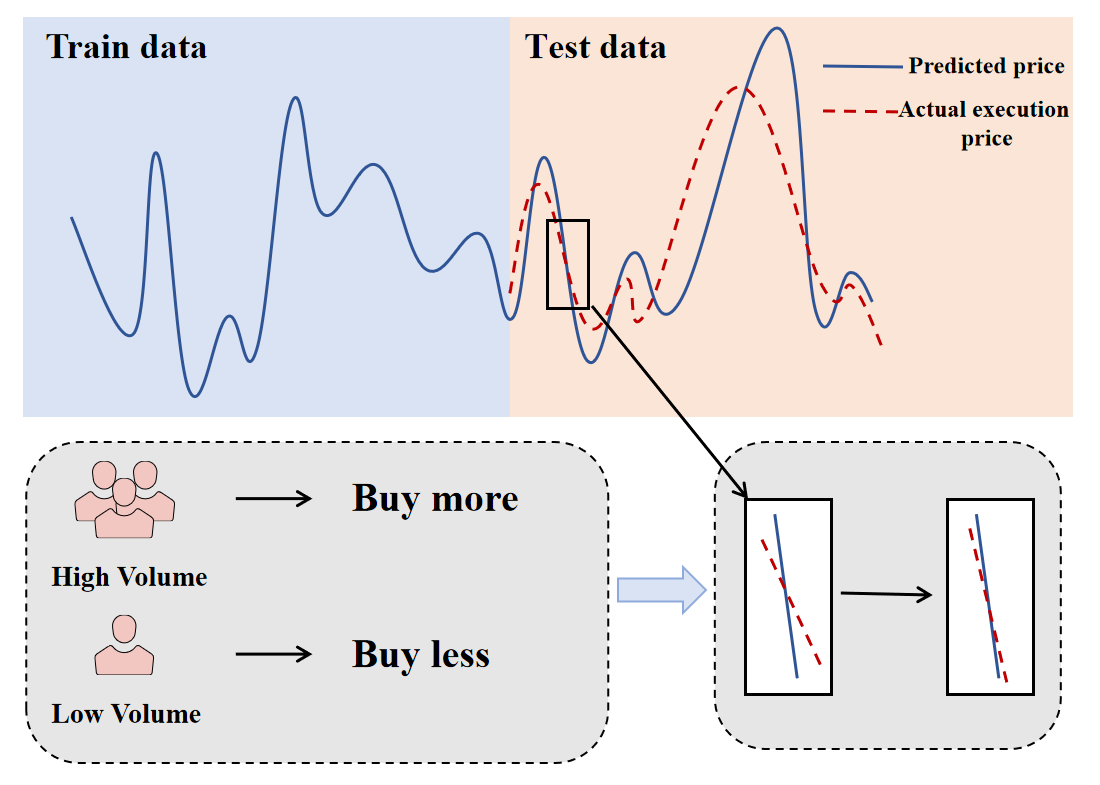
\includegraphics[width=5.67222in,height=3.97986in]{TongjiThesis-master/figures/media/image35.png}

图：通过预测成交量分配购买量来降低滑点损失任务

\textbf{概述}

为了能够构建一个更强大的预测模型来应对非平稳和非线性市场动态，并且能够为大额订单的执行决策提供指导。生成式自回归模型（如Transformers\textsuperscript{{[}6{]}}或Autoformer\textsuperscript{{[}7{]}}等融合变分自编码器的结构）正展现出卓越的预测潜力。这些模型利用了深度神经网络中的创新架构，如自注意力机制，以捕捉金融时间序列中的复杂非线性模式和多尺度依赖关系。此外，由于生成模型能够输出未来分布的概率预测而非单一的确定性值，与传统方法相比，它们能够更全面地量化未来的不确定性，实践经验也证明了深度生成模型的优势，尤其在预测资产价格和波动性方面\textsuperscript{{[}8{]}}。

为解决非平稳市场中对适应性与预测性执行框架的迫切需求，本文提出了一种新型的动态VWAP执行框架，该框架核心在于有机融合了两大关键模块，旨在实现商品期货交易中的动态订单拆分及滑点减少：其一，构建基于Student-t变分自编码器（VAE）与基于自回归解码器的预测模型，负责在随机市场条件下预测未来交易量轨迹和动态参与计划的概率分布，为订单的初步调度提供量化基础；其二，在此预测模型的基础上，进一步引入了多智能体对抗性（Multi-Agent
Adversarial，MAA）交易方向性信号生成器，通过在多个模型骨干和预测时段间的协作学习，从市场中提取并生成鲁棒且时间一致的方向性交易信号，以实时优化订单执行并提升对市场变化的响应能力。

通过联合建模金融数据的潜在结构并利用重尾分布下的概率预测，本文开发了一个基于预测的执行框架，该框架整合了数据表示、潜在空间建模、序列预测以及商品期货市场中的自适应订单拆分等各个环节。旨在弥合预测准确性和实时执行性能之间的差距。通过在18个期货合约、不同市场领域及时间粒度上进行广泛的实验验证，所提方法在滑点控制、VWAP对齐、收益效率及风险调整后稳定性等方面，显著优于传统规则基策略（如MACD\textsuperscript{{[}9{]}}等）。这些发现进一步证实

了生成式自回归模型可以作为复杂金融环境中智能执行基础工具的实际潜力。

\textbf{研究动机}

\subsubsection{\texorpdfstring{\textbf{1.1.1静态}VWAP\textbf{成交量假设无法适应不断变化的微观结构}}{1.1.1静态VWAP成交量假设无法适应不断变化的微观结构}}

传统VWAP依赖于历史成交量平均值来指导订单调度，其核心假设是未来的日内成交量分布将与历史模式保持一致。然而，这种静态假设忽略了市场的动态演变，不仅无法捕捉流动性、订单簿结构及波动性的实时变化，更重要的是，它完全忽视了对未来市场微观结构变化的预期能力。因此，在趋势性或高波动性市场中，固定调度策略表现不佳，导致订单执行效率低下及滑点的增加。这种方法的本质缺陷在于其事后追随的性质------它试图匹配一个已经形成的平均模式，而非主动适应和预测尚未发生的市场行为。这使其在面对突发事件、信息冲击或由中高频交易驱动的瞬时流动性时，显得尤为被动和脆弱。

\subsubsection{\texorpdfstring{\textbf{1.1.2缺乏基于预测的动态调度机制}}{1.1.2缺乏基于预测的动态调度机制}}

大多数当前的执行框架并未纳入对成交量或价格走势的前瞻性预测。这一局限性导致策略无法适应实时市场结构变化。在大额订单中，错过成交量峰值或与价格走势不匹配，可能导致执行效率低下和成本增加。

\textbf{本文贡献}

\subsubsection{\texorpdfstring{\textbf{1.2.1基于变分自编码器的动态}VWAP\textbf{执行策略预测模型研究}}{1.2.1基于变分自编码器的动态VWAP执行策略预测模型研究}}

每个时间戳的成交量和价格被建模为从Student-t分布中条件采样得到。首先使用变分自编码器（VAE）将历史价格和成交量序列压缩到潜在空间表示中，以捕捉结构性模式。随后，采用自回归模块对潜在变量的未来轨迹进行预测，同时预测成交量路径和价格趋势。这些预测结果被输入到动态VWAP调度器中，该调度器实时调整订单拆分比例，以与预测的成交量密度和价格预期保持一致，从而避免低流动性时段并优先在有利时段执行交易。

\textbf{1.2.2兼具宏观微观特征的基于}MAA\textbf{信号生成器的研究}

一种多智能体对抗（MAA）方向性信号生成策略被引入，用于从历史价格轨迹中提取异质性趋势特征，从而生成时间一致且方向敏感的入场和出场信号。信号决策过程利用预测价格变动幅度相对于当前价格的大小，同时基于近期价格分布中统计百分位数动态确定买入和卖出阈值。

该机制通过自适应阈值调整和偏差校正得到强化，从而降低噪声敏感性并保持信号稳健性。实证结果验证了该设计的有效性。如，在ag9999（15分钟买入）设置下，MAA生成的信号数量（超过80次触发）显著多于传统指标（如
MACD）以及深度学习基线模型（iTransformer、FiTS、PatchTST），后者通常仅产生
60--70 次信号。这种较高的信号活跃度并不意味着盲目的过度交易，而是反映了
MAA
所具备的动态适应机制：模型能够根据市场条件主动调整交易方向，从而在市场切换和波动加剧时保持较高的灵敏度与反应速度。

该机制通过自适应阈值调整与偏差校正强化了模型的及时响应能力，使 MAA
能在市场切换或波动加剧时迅速调整交易节奏与方向。实证显示，MAA
在日均收益上显著优于各类基线；以 AP9999 为例，在多种频率配置下 MAA
的日均收益明显高于 iTransformer
等次优模型，表明其在捕捉短周期可交易机会与提高资金使用效率方面具有优势。

同时， MAA 的最大回撤普遍低于 MACD 和多数基线（在某些 60min 配置下 MAA
的最大回撤约 0.10，而 MACD可高达
0.25），且回撤分布更为集中、左尾更短，极端亏损概率更低，说明其在提高收益的同时能更好地控制下行风险。
因此，实验结果支持这样的因果链：及时响应的信号生成与动态执行机制，是 MAA
能同时实现更高日均收益与更低最大回撤的关键。

\textbf{1.2.3模拟交易环境中的实证}

为了评估所提方法的实际效益，在实验中使用历史市场数据和相同的交易信号进行了比较实验。基准策略采用传统的静态VWAP，而模型则整合了VAE-AR预测和动态调度。执行指标如滑点偏差、VWAP对齐度和订单成交效率均被记录。对ni9999合约（多头方向）的实证评估表明，预测执行框架在不同信号频率下可将滑点改善约80\%--160\%（滑点定义见4.2.1滑点计算方法）。具体而言，在15分钟/15分钟配置下，MAA策略实现平均滑点为+0.69（Transformer），而传统MACD基准方法的平均滑点为-0.22。这相当于相对改善约131.8\%，有效将成本转化为执行优势。在更高时间分辨率下，如30分钟/30分钟设置，MAA的滑点为+0.81，而MACD为-1.82，相对改善144.5\%。同样，在60分钟/60分钟场景下，MAA的滑点为+0.31，与iTransformer的-1.71相比具有明显优势，相对改善约123.7\%。这些收益并非单纯的统计现象，而是转化为实际交易成本的显著降低，并与理论VWAP基准的契合度明显提升。这些结果凸显了MAA在不同时间粒度下维持良好成交质量的能力，尤其在高波动性或流动性碎片化的市场环境中。这种优势的一致性进一步证实了模型在实际算法执行环境中方法的稳健性。

\section{6.2 相关工作}

\begin{enumerate}
\def\labelenumi{\arabic{enumi}.}
\item
  \textbf{复杂市场环境下的自适应VWAP}
\end{enumerate}

随着高频交易和程序化交易在商品期货等波动性市场中的普及，VWAP已成为机构执行策略中经典但日益受限的基准指标\textsuperscript{{[}3{]},{[}13{]}}。Almgren-Chriss模型虽然为VWAP在临时市场影响下提供了理论最优性基础，但其主要基于对市场影响的特定假设\textsuperscript{{[}14{]}}。然而，在实际市场中，当存在永久性价格影响和复杂的非线性特征时，最优执行路径将显著偏离简化的VWAP策略，这凸显了传统模型在复杂环境下的局限性。

尽管静态VWAP具有分析上的可处理性，但在动态演变的市场微结构中，其响应能力不足\textsuperscript{{[}16{]}}。为克服这一局限，动态VWAP（Dynamic
VWAP,
DVWAP）的概念应运而生，旨在通过实时调整执行策略以适应市场变化。其发展初期，Almgren和Chriss在最优执行领域奠定了重要理论基础\textsuperscript{{[}14{]}}，同时Bialkowski等也提出了一种动态分解日内交易量的新方法\textsuperscript{{[}4{]}}，该方法通过分离市场共同波动与个股特异性波动，显著提升了VWAP策略的执行精度。这些早期尝试共同推动了VWAP策略从静态向适应性的关键转变。随着研究的深入，近期研究通过整合成交量预测、订单特征及强化学习（如LSTM、M3T）来调整执行计划并减少滑点\textsuperscript{{[}17{]}}。然而，这些改进往往缺乏将预测、调度与执行相结合的统一框架，导致其在碎片化流动性与高频噪声环境下的鲁棒性受限。

鉴于上述挑战，现有VWAP策略的实际有效性严重依赖于其对复杂市场变化的感知与适应能力。目前的研究在整合多源信息、实现预测与执行的无缝联动，以及确保在高波动性环境下的执行稳健性方面仍面临显著空白。因此，迫切需要一种能够更全面地融合预测、调度与执行，并能有效应对碎片化流动性与高频噪声的统一框架。

%\begin{enumerate}
%\def\labelenumi{\arabic{enumi}.}
%\setcounter{enumi}{1}
%\item
  \textbf{自回归Transformer在金融预测中的应用}
%\end{enumerate}

近年来，自回归Transformer架构在金融时间序列建模中的应用迅速发展，这得益于其能够捕捉噪声市场数据中的长程依赖关系和复杂时间模式。自注意力机制作为这些模型的核心组件，能够在变长序列中实现动态上下文建模，使Transformer特别适合处理金融信号的不规则性和波动性。诸如时序融合Transformer等架构通过整合领域特定的归纳偏置（如门控机制和变量选择网络）来提升多时段预测精度\textsuperscript{{[}18{]}}，此外，Transformer模型已被适配以捕捉跨资产依赖关系，在股票回报预测任务中表现优于资产特定模型\textsuperscript{{[}19{]}}。

除了单变量或多变量价格建模外，基于Transformer的框架在多模态学习方面也展现出强大的潜力。特别是，将文本信息（如财务新闻或社交媒体情绪）与历史价格数据相结合的研究已证明了显著的预测改进。GPT风格架构的灵活性使其能够有效解析非结构化自然语言并生成与市场相关的表示\textsuperscript{{[}20{]},{[}21{]},{[}22{]}}，从而丰富下游预测模型。

尽管取得了这些进展，仍存在若干挑战。金融数据集通常噪声较大、维度较高且标签稀疏，导致过拟合和泛化问题，尤其是在模型基于有限历史数据进行训练时\textsuperscript{{[}23{]},{[}24{]}}。此外，标准Transformer架构在处理非常长的序列时会遇到计算瓶颈\textsuperscript{{[}25{]}}，而多步预测中的自回归推理可能因累积误差传播和延迟限制而受限\textsuperscript{{[}26{]}}。尽管已提出结构创新如Autoformer通过利用分解式注意力机制和自相关机制来缓解这些问题\textsuperscript{{[}7{]}}，但此类方案通常以增加架构复杂性为代价。

综上所述，自回归Transformer（特别是类似GPT的解码器式模型以及注意力增强的编码器-解码器变体）为建模复杂金融系统提供了强大的范式。然而，其在实践中的成功部署需要谨慎的正则化、基于领域知识的架构定制，以及严格的验证，以确保在真实市场条件下的稳健性。

\begin{enumerate}
\def\labelenumi{\arabic{enumi}.}
\setcounter{enumi}{2}
\item
  \textbf{利用Student-t分布建模尾部风险}
\end{enumerate}

对金融极端事件的稳健建模促使人们越来越多地采用重尾分布，特别是Student-t分布，作为对高斯假设的替代方案。实证研究证实，资产回报具有尖峰和重尾特征，而t分布可通过调整自由度灵活适应这些特征\textsuperscript{{[}27{]}}。这改善了尾部概率估计并减少了风险度量中的系统性偏差，例如风险价值（VaR）\textsuperscript{{[}28{]}}。

而多元t分布和t-copula在捕捉资产之间的尾部依赖性方面优于Gaussian-copula\textsuperscript{{[}29{]}}，尤其是在承受市场压力下\textsuperscript{{[}30{]}}。时间序列模型如t-GARCH和t-EGARCH进一步利用这些特性来改进波动率建模\textsuperscript{{[}31{]}}，而贝叶斯和HMM模型则利用t-likelihoods进行异常情况下的稳健估计\textsuperscript{{[}32{]}}。

尽管t-distributions的对称性假设限制了它对偏态
资产（如隐含波动率）的建模能力，导致极值分布或非对称拉普拉斯分布等替代方案可能更优，但
t-distributions仍然是一个实用的基准。它可以与波动率模型或生成模型（如VAE、GAN）集成，从而在金融预测系统中实现稳健性与计算可扩展性的平衡。

\section{6.3 算法机制}\label{ux7b97ux6cd5ux673aux5236-2}

本研究的目标是为未来离散时间区间
\includegraphics[width=0.16667in,height=0.16667in]{TongjiThesis-master/figures/media/image36.png}内的总订单规模
\includegraphics[width=0.33333in,height=0.22917in]{TongjiThesis-master/figures/media/image37.png}设计一个最优执行策略。该策略由订单集合
\includegraphics[width=0.83333in,height=0.22917in]{TongjiThesis-master/figures/media/image38.png}
表示，其中
\includegraphics[width=0.79861in,height=0.5in]{TongjiThesis-master/figures/media/image39.png}，该策略的目标是能够最小化交易过程中所产生的总滑点。其核心观点是在给定时间
\includegraphics[width=\linewidth,height=0.16667in,keepaspectratio]{TongjiThesis-master/figures/media/image40.png}时的最优订单规模
\includegraphics[width=0.16667in,height=0.22917in]{TongjiThesis-master/figures/media/image41.png}应与市场的吸收能力成正比，而吸收能力可通过准确预测未来市场成交量来近似。

为实现这种动态、低成本的算法交易，本研究设计了一个包含两大核心模块的综合性执行框架：（1）基于多智能体对抗（MAA）的信号生成器，其目的是从复杂的市场数据中提取高置信度的、具有方向性的交易时机（即``何时交易、交易方向''）；（2）基于生成式自回归模型的动态订单执行器，其核心是利用Student-t变分自编码器（VAE）和一个自回归的解码器来预测未来成交量分布，目的是在信号触发后，智能地将大额订单拆分到最优的微观时间片上执行（即``如何交易''）。本节将首先陈述算法交易的优化目标，然后依次详细介绍订单执行和信号生成的具体方法。整体框架如图1所示。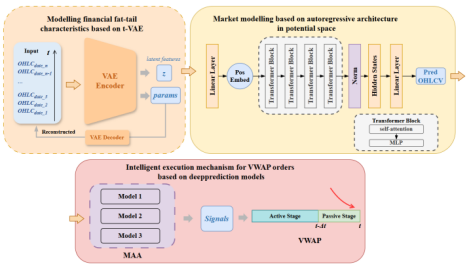
\includegraphics[width=3.25694in,height=1.86111in]{TongjiThesis-master/figures/media/image42.png}

\textbf{图1执行流程框架图}

Fig.1 Procedure of execution

\begin{enumerate}
\def\labelenumi{\arabic{enumi}.}
\item
  \textbf{问题陈述}
\end{enumerate}

本研究的交易框架是假设在给定时间
\includegraphics[width=0.16667in,height=0.25694in]{CTongjiThesis-master/figures/media/image43.png}发出\st{的}交易指令，要求在时间窗口
\includegraphics[width=0.74306in,height=0.22917in]{TongjiThesis-master/figures/media/image44.png}内交易总计
\includegraphics[width=0.33333in,height=0.22917in]{TongjiThesis-master/figures/media/image37.png}的交易量。本文将该窗口划分为
\includegraphics[width=0.16667in,height=0.16667in]{TongjiThesis-master/figures/media/image36.png}个等长的时间区间。在每个
\includegraphics[width=0.70833in,height=0.20833in]{TongjiThesis-master/figures/media/image45.png}区间的开始时刻，总量有一个固定的需要下单总规模
\includegraphics[width=0.16667in,height=0.22917in]{TongjiThesis-master/figures/media/image41.png}。

在经典VWAP执行策略中，常见的做法是将订单数量按成交量比例在各个时间区间内分配。然而，这种分配方式本质上只保证了``均匀参与''，并未直接考虑价格水平的优劣。对于买方而言，在任意区间若能在最低价附近完成交易，其执行成本显然会优于单纯的均值导向。

因此，我们在动态VWAP策略中引入区间最低价
VWAP作为目标，并通过优化问题来体现执行逻辑。设区间
\includegraphics[width=0.10417in,height=0.16667in]{TongjiThesis-master/figures/media/image46.png}的参考价为
\includegraphics[width=0.23958in,height=0.1875in,alt={IMG\_256}]{TongjiThesis-master/figures/media/image47.png}（买方取区间最低价
\includegraphics[width=0.39583in,height=0.15625in,alt={IMG\_256}]{TongjiThesis-master/figures/media/image47.png}，卖方取区间最高价
\includegraphics[width=0.42708in,height=0.15625in,alt={IMG\_273}]{TongjiThesis-master/figures/media/image47.png}），方向参数
\includegraphics[width=1.15625in,height=0.15625in,alt={IMG\_274}]{TongjiThesis-master/figures/media/image47.png}表示买卖方向（买入
\includegraphics[width=0.70833in,height=0.15625in,alt={IMG\_275}]{TongjiThesis-master/figures/media/image47.png}，卖出

\includegraphics[width=0.70833in,height=0.15625in,alt={IMG\_276}]{TongjiThesis-master/figures/media/image47.png}），则订单数量的最优分配可表述为：


\includegraphics[width=3.38889in,height=0.32639in]{TongjiThesis-master/figures/media/image48.png}

(3-1)

其中，第一项

\includegraphics[width=0.77083in,height=0.15625in,alt={IMG\_278}]{TongjiThesis-master/figures/media/image47.png}
衡量实际单量与预期单量之间的差异（数量约束，需尽量最小化），第二项

\includegraphics[width=1.82292in,height=0.1875in,alt={IMG\_279}]{TongjiThesis-master/figures/media/image47.png}
则刻画价格相对参考价的优势（价格目标，需尽量最大化），
\includegraphics[width=0.35417in,height=0.15625in,alt={IMG\_280}]{TongjiThesis-master/figures/media/image47.png}
为平衡系数。通过这种方式，策略不仅能够保证整体成交数量的合理分布，同时在价格层面也能尽量贴近区间的最优成交水平。

研究指出，与正态分布相比，
\includegraphics[width=\linewidth,height=0.16667in,keepaspectratio,alt={IMG\_281}]{TongjiThesis-master/figures/media/image47.png}分布的重尾特性本质上更擅长捕捉金融市场中普遍存在的随机性和极端事件\textsuperscript{{[}33{]},{[}34{]}}。这一特性在构建神经网络模型时提供了关键的先验指导。

为了构建一个能够捕捉金融数据重尾特性的概率模型，我们进行了如下设计。首先，金融数据往往存在较强的波动性，直接使用原始序列容易导致方差不稳定。为此，我们采用对数变换，将数据映射到实数域，从而有效降低整体方差并缓解异方差问题。其次，为捕捉金融市场中常见的``尖峰厚尾''现象，我们选择Student-t分布替代传统的高斯分布，因为它能更好地对极端市场波动进行建模。

我们首先对原始观测序列进行对数变换，以降低整体方差。设

\includegraphics[width=0.75in,height=0.16667in,alt={IMG\_282}]{TongjiThesis-master/figures/media/image47.png}
表示时刻 \emph{t}
的金融指标（如开盘价、收盘价、成交量等），
\includegraphics[width=0.16667in,height=0.16667in,alt={IMG\_283}]{TongjiThesis-master/figures/media/image47.png}是金融指标的维度，定义逐元素运算的对数变换：


\includegraphics[width=1.14583in,height=0.1875in,alt={IMG\_284}]{TongjiThesis-master/figures/media/image47.png}
(3-2)

但是，单一时刻的观测值不足以完整反映市场动态，因此我们引入潜变量

\includegraphics[width=0.40625in,height=0.15625in,alt={IMG\_285}]{TongjiThesis-master/figures/media/image47.png}，它由过去

\includegraphics[width=0.35417in,height=0.15625in,alt={IMG\_286}]{TongjiThesis-master/figures/media/image47.png}
步的历史窗口信息压缩得到：


\includegraphics[width=2.61458in,height=0.20833in,alt={IMG\_287}]{TongjiThesis-master/figures/media/image47.png}
(3-3)

其中

\includegraphics[width=0.79167in,height=0.17708in,alt={IMG\_288}]{TongjiThesis-master/figures/media/image47.png}
表示非线性编码器（如下文3.2节提到的 VAE
编码器），将高维价量序列映射到低维潜变量空间。于是我们定义状态

\includegraphics[width=0.38542in,height=0.15625in,alt={IMG\_289}]{TongjiThesis-master/figures/media/image47.png}
为该潜变量

\includegraphics[width=0.40625in,height=0.15625in,alt={IMG\_290}]{ TongjiThesis-master/figures/media/image47.png}。

基于此，我们提出本文的核心假设：在任意时刻 \emph{t}，给定状态

\includegraphics[width=0.38542in,height=0.15625in,alt={IMG\_291}]{TongjiThesis-master/figures/media/image47.png}
未来

\includegraphics[width=0.375in,height=0.15625in,alt={IMG\_292}]{TongjiThesis-master/figures/media/image47.png}
步的潜变量序列服从一个多元

\includegraphics[width=0.33333in,height=0.15625in,alt={IMG\_293}]{TongjiThesis-master/figures/media/image47.png}
分布：


\includegraphics[width=2.5625in,height=0.16667in,alt={IMG\_294}]{TongjiThesis-master/figures/media/image47.png}
(3-4)

若

\includegraphics[width=0.64583in,height=0.15625in,alt={IMG\_295}]{TongjiThesis-master/figures/media/image47.png}，简化为一步预测：


\includegraphics[width=2.10417in,height=0.15625in,alt={IMG\_296}]{TongjiThesis-master/figures/media/image47.png}
(3-5)

其中，
\includegraphics[width=0.58333in,height=0.15625in,alt={IMG\_297}]{TongjiThesis-master/figures/media/image47.png}
为位置参数，决定分布的中心位置；
\includegraphics[width=0.58333in,height=0.15625in,alt={IMG\_298}]{TongjiThesis-master/figures/media/image47.png}
为尺度矩阵，刻画不同维度之间的相关性及伸缩形状；
\includegraphics[width=0.58333in,height=0.15625in,alt={IMG\_299}]{TongjiThesis-master/figures/media/image47.png}
为自由度参数，用来控制分布尾部的厚度，
\includegraphics[width=0.35417in,height=0.15625in,alt={IMG\_300}]{TongjiThesis-master/figures/media/image47.png}
越小，尾部越厚，更能反映金融数据中极端波动的特性。

未来多步预测的联合分布可通过乘积分解实现：


\includegraphics[width=2.88542in,height=0.19792in,alt={IMG\_301}]{TongjiThesis-master/figures/media/image47.png}
(3-6)

这一分解强调未来每一步的预测依赖于状态

\includegraphics[width=0.38542in,height=0.15625in,alt={IMG\_302}]{TongjiThesis-master/figures/media/image47.png}
和先前生成的潜变量，从而自然适应序列建模。每个条件分布取为多元
Student-t（小写

\includegraphics[width=0.33333in,height=0.15625in,alt={IMG\_303}]{TongjiThesis-master/figures/media/image47.png}），其密度函数为：


\includegraphics[width=0.77083in,height=0.15625in,alt={IMG\_304}]{TongjiThesis-master/figures/media/image47.png}


\includegraphics[width=3.19792in,height=0.36458in,alt={IMG\_305}]{TongjiThesis-master/figures/media/image47.png}
(3-7)

该分布具备厚尾特性（小

\includegraphics[width=0.35417in,height=0.15625in,alt={IMG\_306}]{TongjiThesis-master/figures/media/image47.png}
时），相比正态分布更能刻画金融市场中的极端行情。在预测潜变量序列

\includegraphics[width=0.53125in,height=0.15625in,alt={IMG\_307}]{TongjiThesis-master/figures/media/image47.png}
后，首先通过 VAE 解码器映射得到对数空间的预测值：


\includegraphics[width=2.17708in,height=0.17708in,alt={IMG\_308}]{TongjiThesis-master/figures/media/image47.png}
(3-8)

随后，再通过指数反变换得到原始指标空间中的预测：


\includegraphics[width=2.45833in,height=0.17708in,alt={IMG\_309}]{TongjiThesis-master/figures/media/image47.png}
(3-9)

这一过程确保了预测结果的非负性，并保持与原始金融指标的可比性。

简而言之，当未来时间步长可用（如在训练过程中）时，可以利用完整上下文条件来实现更准确的参数估计。相反，在未来预测时段的推理过程中，这种形式化方法能够实现对对数转换后市场状态序列的逐步自回归生成。

接下来将详细说明如何使用变分自编码器将原始时间序列数据
\includegraphics[width=0.20833in,height=0.22917in,alt={IMG\_310}]{TongjiThesis-master/figures/media/image47.png}拟合到对数
\includegraphics[width=0.10417in,height=0.16667in,alt={IMG\_311}]{TongjiThesis-master/figures/media/image47.png}分布，从而获得自回归公式所需的参数。

\begin{enumerate}
\def\labelenumi{\arabic{enumi}.}
\setcounter{enumi}{1}
\item
  \textbf{潜在空间建模与自回归预测}
\end{enumerate}

\textbf{3.2.1使用Student-t变分自编码器拟合时间序列数据}

为了获得条件t分布
\includegraphics[width=0.91667in,height=0.15625in,alt={IMG\_312}]{TongjiThesis-master/figures/media/image47.png}的参数
\includegraphics[width=1.45833in,height=0.15625in,alt={IMG\_313}]{TongjiThesis-master/figures/media/image47.png}，如在上文中所述，我们采用了一种专门的变分自编码器（VAE）。该VAE旨在学习金融时间序列的稳健表示，它通过Student-t分布来明确地建模潜在空间。考虑到原始经济数据（如价格和成交量）的统计特性在对数变换后表现更佳，模型先对输入序列进行对数变换，以稳定方差并缓解偏态问题。其整体架构依然遵循编码器--解码器范式，具体的编码器与解码器可以选用
Transformer、LSTM
或其他适合捕捉复杂时间依赖关系的神经网络结构，从而在保持灵活性的同时，更好地适应不同数据特征。

将编码器网络记为
\includegraphics[width=0.67708in,height=0.25in,alt={IMG\_314}]{TongjiThesis-master/figures/media/image47.png}，该模型负责将输入的最小间隔数据张量
\includegraphics[width=0.20833in,height=0.21875in,alt={IMG\_315}]{TongjiThesis-master/figures/media/image47.png}映射到近似后验分布的参数。与通常假设后验为高斯分布的标准VAE不同，编码器生成多元Student-t分布的参数：位置向量
\includegraphics[width=0.20833in,height=0.25in,alt={IMG\_316}]{TongjiThesis-master/figures/media/image47.png}、通过其对数表示的尺度向量
\includegraphics[width=0.40625in,height=0.25in,alt={IMG\_317}]{TongjiThesis-master/figures/media/image47.png}，以及自由度，同样以对数形式表示的
\includegraphics[width=0.375in,height=0.25in,alt={IMG\_318}]{TongjiThesis-master/figures/media/image47.png}。为了确保优化过程可微分，采用了针对
\includegraphics[width=\linewidth,height=0.16667in,keepaspectratio,alt={IMG\_319}]{TongjiThesis-master/figures/media/image47.png}分布适配的重新参数化技巧。一个潜在样本
\includegraphics[width=0.16667in,height=0.21875in,alt={IMG\_320}]{TongjiThesis-master/figures/media/image47.png}通过以下变换生成：


\includegraphics[width=1.5in,height=0.25in,alt={IMG\_321}]{TongjiThesis-master/figures/media/image47.png}
(3-10)

其中

\includegraphics[width=0.14583in,height=0.16667in,alt={IMG\_322}]{TongjiThesis-master/figures/media/image47.png}是从标准Student-t分布中抽取的随机变量。该采样过程的自由度计算为：


\includegraphics[width=1.52083in,height=0.25in,alt={IMG\_323}]{TongjiThesis-master/figures/media/image47.png}。
(3-11)

而解码器网络
\includegraphics[width=0.70833in,height=0.21875in,alt={IMG\_324}]{TongjiThesis-master/figures/media/image47.png}则执行的是反向操作，它从潜在空间中采样得到的变量
\includegraphics[width=0.16667in,height=0.21875in,alt={IMG\_325}]{TongjiThesis-master/figures/media/image47.png}出发，试图重建原始输入数据，从而产生
\includegraphics[width=0.21875in,height=0.25in,alt={IMG\_326}]{TongjiThesis-master/figures/media/image47.png}。整个模型通过端到端的方式进行训练，目标是最小化一个复合损失函数
\includegraphics[width=0.58333in,height=0.15625in,alt={IMG\_327}]{TongjiThesis-master/figures/media/image47.png}，该函数源自负的证据下界（negative
ELBO）\textsuperscript{{[}35{]}}。该损失函数合理地结合了数据重构项和正则化项，以实现重构效果与潜在空间约束之间的平衡。它由三部分加权构成。其一，重构损失
\includegraphics[width=0.375in,height=0.21875in,alt={IMG\_328}]{TongjiThesis-master/figures/media/image47.png}根据数据的特点进行设计：对于价格相关的特征（如开盘价、最高价、最低价和收盘价），对异常值则采用更具鲁棒性的Huber损失，而对于成交量相关的特征，则使用均方误差（MSE），确保潜在表示能有效还原原始输入信息。

其二，损失函数中的正则化成分对塑造潜在空间至关重要。它主要由学习到的后验分布
\includegraphics[width=0.6875in,height=0.25in,alt={IMG\_329}]{TongjiThesis-master/figures/media/image47.png}与固定的先验分布
\includegraphics[width=0.375in,height=0.21875in,alt={IMG\_330}]{TongjiThesis-master/figures/media/image47.png}之间的Kullback-Leibler（KL）散度组成。将该先验定义为标准多元Student's-t分布，以在潜在空间中引入重尾特性。由于两个
\includegraphics[width=\linewidth,height=0.16667in,keepaspectratio,alt={IMG\_331}]{TongjiThesis-master/figures/media/image47.png}分布之间KL散度的解析复杂性，相应的采用蒙特卡洛方法进行估计，通过后验分布的样本平均
\includegraphics[width=1.58333in,height=0.25in,alt={IMG\_332}]{TongjiThesis-master/figures/media/image47.png}的值。

其三，为了进一步强化期望的尾部行为，引入额外的惩罚项
\includegraphics[width=1.16667in,height=0.25in,alt={IMG\_333}]{TongjiThesis-master/figures/media/image47.png}，该项明确鼓励学习到的自由度与先验分布的自由度匹配。

最终目标函数是这三个组分的加权和：


\includegraphics[width=2.8125in,height=0.25in,alt={IMG\_334}]{TongjiThesis-master/figures/media/image47.png}
(3-12)

其中
\includegraphics[width=0.16667in,height=0.20833in,alt={IMG\_335}]{TongjiThesis-master/figures/media/image47.png}和

\includegraphics[width=0.14583in,height=0.1875in,alt={IMG\_336}]{TongjiThesis-master/figures/media/image47.png}是超参数，用于平衡重建保真度与正则化强度。通过最小化该目标函数，编码器学会将任何市场状态
\includegraphics[width=0.20833in,height=0.21875in,alt={IMG\_337}]{TongjiThesis-master/figures/media/image47.png}映射到最能代表它的
\includegraphics[width=0.10417in,height=0.16667in,alt={IMG\_338}]{TongjiThesis-master/figures/media/image47.png}分布参数，从而为提出的自回归模型提供必要的组件。

\textbf{3.2.2自回归 Transformer 预测器}

在获得 VAE 学习到的潜变量表示之后，我们进一步利用自回归 Transformer（AR
Transformer）对时间序列的动态进行建模。其核心思想是：VAE
提供稳健的潜变量表征

\includegraphics[width=0.41667in,height=0.15625in,alt={IMG\_339}]{TongjiThesis-master/figures/media/image47.png}，而
AR Transformer
在原始观测空间（OHLCV）上对未来走势进行预测，从而为订单拆分提供依据。

不同于严格的一步步自回归预测，本研究采用带重叠的滑动窗口方式来加速训练与收敛。具体而言，给定一个长度为

\includegraphics[width=0.38542in,height=0.15625in,alt={IMG\_340}]{TongjiThesis-master/figures/media/image47.png}
的输入窗口

\includegraphics[width=0.63542in,height=0.15625in,alt={IMG\_341}]{TongjiThesis-master/figures/media/image47.png}，模型直接预测与之对齐的未来窗口：


\includegraphics[width=1.67708in,height=0.16667in,alt={IMG\_342}]{TongjiThesis-master/figures/media/image47.png}
(3-13)

其中

\includegraphics[width=0.89583in,height=0.16667in,alt={IMG\_343}]{TongjiThesis-master/figures/media/image47.png}
表示预测得到的连续片段。通过在训练过程中不断滑动窗口并对齐目标区间，模型能够在一次训练中同时学习多个未来时刻的预测，从而提升效率与稳定性。

随后，预测得到的序列

\includegraphics[width=0.89583in,height=0.16667in,alt={IMG\_344}]{TongjiThesis-master/figures/media/image47.png}
会再次通过 VAE 编码器转化为潜变量

\includegraphics[width=0.88542in,height=0.16667in,alt={IMG\_345}]{TongjiThesis-master/figures/media/image47.png}，以保证预测在潜在空间中的一致性与可递推性。这种设计使得
VAE 与 AR Transformer
相互协作：前者负责提供鲁棒的分布式潜变量建模，后者负责时间序列上的动态预测。

在训练过程中，AR Transformer 的目标是使预测序列

\includegraphics[width=0.89583in,height=0.16667in,alt={IMG\_346}]{TongjiThesis-master/figures/media/image47.png}
尽可能贴近真实观测
\includegraphics[width=0.89583in,height=0.15625in,alt={IMG\_347}]{TongjiThesis-master/figures/media/image47.png}，因此优化目标采用均方误差（MSE）：


\includegraphics[width=2.625in,height=0.22917in,alt={IMG\_348}]{TongjiThesis-master/figures/media/image47.png}(3-14)

通过这种方式，模型在保证时序依赖性的同时，有效提升了训练效率，并能更好地适应金融时间序列的复杂动态。

\begin{enumerate}
\def\labelenumi{\arabic{enumi}.}
\setcounter{enumi}{2}
\item
  \textbf{下单策略}
\end{enumerate}

本研究的订单拆分策略是一个宏观信号触发、微观智能执行的两层架构。宏观层面，信号生成器（如后文所述的MAA模型）负责在较长时间尺度（如15分钟、半小时、一天）上监测市场，并生成``买入''、``卖出''或``持仓''的决策。微观层面，一旦宏观信号在t时刻触发了一个总规模为
\includegraphics[width=0.55208in,height=0.15625in,alt={IMG\_349}]{TongjiThesis-master/figures/media/image47.png}的交易指令，订单执行器便会启动。它的核心任务是在该执行窗口（如15分钟等）内，依据VAE
与自回归 Transformer（AR
Transformer）联合建模的预测结果，将
\includegraphics[width=0.55208in,height=0.15625in,alt={IMG\_350}]{TongjiThesis-master/figures/media/image47.png}动态地分配到各个子时段中。这种设计的目的是确保交易行为与市场流动性动态匹配，从而降低滑点。本节将详细阐述微观层面的动态数量计算与执行保障机制。

\begin{enumerate}
\def\labelenumi{\arabic{enumi}.}
\item
  \textbf{动态订单数量计算}
\end{enumerate}

在总执行窗口
\includegraphics[width=0.33333in,height=0.20833in,alt={IMG\_351}]{TongjiThesis-master/figures/media/image47.png}内的每个时间间隔
\includegraphics[width=\linewidth,height=0.16667in,keepaspectratio,alt={IMG\_352}]{TongjiThesis-master/figures/media/image47.png}的开始时，主要任务是计算该特定间隔的目标订单数量
\includegraphics[width=0.16667in,height=0.21875in,alt={IMG\_353}]{TongjiThesis-master/figures/media/image47.png}。设
\includegraphics[width=0.29167in,height=0.27083in,alt={IMG\_354}]{TongjiThesis-master/figures/media/image47.png}表示在间隔
\includegraphics[width=\linewidth,height=0.16667in,keepaspectratio,alt={IMG\_355}]{TongjiThesis-master/figures/media/image47.png}开始时仍需执行的剩余数量。

本方法将从一个简单且稳健的基线开始：均匀分割。在缺乏任何预测信息的情况下，最直接的策略是将剩余订单数量均匀分配到剩余的时间区间中：


\includegraphics[width=1.14583in,height=0.44792in,alt={IMG\_356}]{TongjiThesis-master/figures/media/image47.png}
(3-15)

然而，这个静态基线策略无法对市场流动性的变化做出响应。为此，本文利用
VAE-AR Transformer
预测框架，在时间点
\includegraphics[width=\linewidth,height=0.16667in,keepaspectratio,alt={IMG\_357}]{TongjiThesis-master/figures/media/image47.png}预测执行窗口内后续所有时间区间的市场成交量分布，即
\includegraphics[width=1.16667in,height=0.27083in,alt={IMG\_358}]{TongjiThesis-master/figures/media/image47.png}。基于这些预测信息，为当前时段分配一个动态参与权重
\includegraphics[width=0.1875in,height=0.21875in,alt={IMG\_359}]{TongjiThesis-master/figures/media/image47.png}:


\includegraphics[width=0.75in,height=0.70833in,alt={IMG\_360}]{TongjiThesis-master/figures/media/image47.png}
(3-16)

该权重代表当前区间内预计占总剩余市场成交量比例的预测值。最终目标数量
\includegraphics[width=0.16667in,height=0.21875in,alt={IMG\_361}]{TongjiThesis-master/figures/media/image47.png}通过将该权重应用于总剩余订单规模计算得出，实质上形成了一个类似VWAP（成交量加权平均价格）的定价方案：


\includegraphics[width=0.79167in,height=0.27083in,alt={IMG\_362}]{TongjiThesis-master/figures/media/image47.png}
(3-17)

这种动态调整使策略能够在预计流动性较高的时期更积极地交易，而在预计流动性较低的时期则更被动地交易，从而最大限度减少市场的成交量对于成交概率的影响。为了确保稳健性，在模型预测的未来成交量微不足道（
\includegraphics[width=0.6875in,height=0.29167in,alt={IMG\_363}]{TongjiThesis-master/figures/media/image47.png}）或历史数据不足以进行可靠预测的情况下，策略会自动切换到均匀分割基准，以确保稳定性。

\begin{enumerate}
\def\labelenumi{\arabic{enumi}.}
\setcounter{enumi}{1}
\item
  \textbf{时间间隔内的执行策略与完成性保障}
\end{enumerate}

一旦确定了当前时间间隔（如持续时间为
\includegraphics[width=0.20833in,height=0.1875in,alt={IMG\_364}]{TongjiThesis-master/figures/media/image47.png}的一分钟）的目标数量
\includegraphics[width=0.16667in,height=0.21875in,alt={IMG\_365}]{ TongjiThesis-master/figures/media/image47.png}，接下来面临的挑战是如何在保证完成的前提下高效执行该目标。主动下达限价单虽能降低成本，但存在无法成交的风险。为缓解这一问题，在每个时间间隔内采用基于时间的两阶段执行逻辑，即将时间间隔
\includegraphics[width=0.20833in,height=0.1875in,alt={IMG\_366}]{ TongjiThesis-master/figures/media/image47.png}划分为两个阶段：持续时间为
\includegraphics[width=0.47917in,height=0.1875in,alt={IMG\_367}]{ TongjiThesis-master/figures/media/image47.png}的主动执行阶段，以及持续时间为
\includegraphics[width=0.20833in,height=0.1875in,alt={IMG\_368}]{ TongjiThesis-master/figures/media/image47.png}的被动完成阶段。如在60秒的时间间隔中，前50秒可用于主动执行，剩余10秒用于被动完成。

Phase1:主动执行阶段

在初始的
\includegraphics[width=0.47917in,height=0.1875in,alt={IMG\_369}]{ TongjiThesis-master/figures/media/image47.png}期间，策略依托
VAE 与 AR Transformer
的预测结果，对未来时间段的市场成交量进行动态管理。当预测显示当前时段流动性较高时，策略会主动分配更多订单以快速执行，填充数量
\includegraphics[width=0.16667in,height=0.21875in,alt={IMG\_370}]{ TongjiThesis-master/figures/media/image47.png}。具体执行上，策略通常采用限价单，其``主动''体现在我们根据预测结果主动选择价格与时机来挂单，而非被动等待市场波动。这种方式既能利用预测的市场容量降低冲击成本，又能通过价格控制减少显性交易费用。

Phase2:被动完成阶段

在主动阶段结束时，任何未执行的
\includegraphics[width=0.16667in,height=0.21875in,alt={IMG\_371}]{ TongjiThesis-master/figures/media/image47.png}部分，将其表示为
\includegraphics[width=0.47917in,height=0.27083in,alt={IMG\_372}]{ TongjiThesis-master/figures/media/image47.png}，必须在剩余的
\includegraphics[width=0.20833in,height=0.1875in,alt={IMG\_373}]{ TongjiThesis-master/figures/media/image47.png}内执行，以确保每个间隔的目标得以实现。为了避免下达单个可能影响较大的市场订单，将其拆分为一系列较小的``子''订单。这些子订单根据几何级数模型进行分发。随着区间截止时间的临近，订单规模逐渐减小。假设完成阶段
\includegraphics[width=0.20833in,height=0.1875in,alt={IMG\_374}]{ TongjiThesis-master/figures/media/image47.png}包含
\includegraphics[width=0.16667in,height=0.16667in,alt={IMG\_375}]{ TongjiThesis-master/figures/media/image47.png}个离散的发送时间戳。若首个子订单的规模为
\includegraphics[width=0.16667in,height=0.21875in,alt={IMG\_376}]{ TongjiThesis-master/figures/media/image47.png}，且公比为
\includegraphics[width=0.14583in,height=0.16667in,alt={IMG\_377}]{ TongjiThesis-master/figures/media/image47.png}（其中0\textless{}
\includegraphics[width=0.14583in,height=0.16667in,alt={IMG\_378}]{ TongjiThesis-master/figures/media/image47.png}\textless1），则订单规模序列将为
\includegraphics[width=1.4375in,height=0.27083in,alt={IMG\_379}]{ TongjiThesis-master/figures/media/image47.png}。为确保总交易量与未成交量匹配，该几何级数之和必须等于
\includegraphics[width=0.47917in,height=0.27083in,alt={IMG\_380}]{ TongjiThesis-master/figures/media/image47.png}。


\includegraphics[width=1.75in,height=0.47917in,alt={IMG\_381}]{ TongjiThesis-master/figures/media/image47.png}
(3-18)

由此可计算初始订单规模
\includegraphics[width=0.16667in,height=0.21875in,alt={IMG\_382}]{ TongjiThesis-master/figures/media/image47.png}，进而确定所有子订单。这些较小的订单随后以市价单形式执行，以确保其成交。这种``渐消''策略在完成阶段初期放置较大订单块，并逐渐减少至结束。这种精细控制旨在缓解因间隔结束时单个大规模``恐慌''订单引发的价格冲击和信号风险，从而实现计划数量
\includegraphics[width=0.16667in,height=0.21875in,alt={IMG\_383}]{ TongjiThesis-master/figures/media/image47.png}的更平滑、更稳健的完成。

\begin{enumerate}
\def\labelenumi{\arabic{enumi}.}
\setcounter{enumi}{3}
\item
  \textbf{基于多智能体对抗框架的信号生成器}
\end{enumerate}

宏观交易信号是整个动态 VWAP
策略的触发源，其质量直接决定了后续订单执行的有效性。然而，金融市场价格与流动性往往具有显著的高波动性和非平稳特征，使得传统单模型预测方法容易陷入过拟合或缺乏鲁棒性。

为此，本文提出了一种基于多智能体对抗框架（MAA, Multi-Agent
Adversarial）的信号生成器。其基本思路是：通过多个生成器和判别器的对抗博弈，形成一个动态演化的预测环境，再结合蒸馏与集成机制，提高预测的鲁棒性与泛化性能。本节将从多智能体对抗训练、知识蒸馏与优化机制以及集成预测与信号生成三个层次展开论述。


\includegraphics[width=3.25in,height=1.625in,alt={IMG\_384}]{ TongjiThesis-master/figures/media/image47.png}\textbf{图2多智能体对抗性（MAA）训练流程}

Fig.2 Multi Agent Adversarial(MAA) training procedure

\begin{enumerate}
\def\labelenumi{\arabic{enumi}.}
\item
  \textbf{多智能体对抗训练}
\end{enumerate}

图2中展示了多智能体对抗（MAA）的训练流程。在MAA框架中，设有
\includegraphics[width=0.375in,height=0.15625in,alt={IMG\_385}]{ TongjiThesis-master/figures/media/image47.png}个生成器

\includegraphics[width=1.17708in,height=0.15625in,alt={IMG\_386}]{ TongjiThesis-master/figures/media/image47.png}
与 N 个判别器

\includegraphics[width=1.21875in,height=0.15625in,alt={IMG\_387}]{ TongjiThesis-master/figures/media/image47.png}。生成器的作用是利用输入的历史窗口

\includegraphics[width=0.54167in,height=0.19792in,alt={IMG\_388}]{ TongjiThesis-master/figures/media/image47.png}
对未来一段时间的市场走势进行预测，包括连续值（如价格、成交量）的回归预测
\includegraphics[width=0.46875in,height=0.16667in,alt={IMG\_389}]{ TongjiThesis-master/figures/media/image47.png}和市场趋势方向的分类预测

\includegraphics[width=0.47917in,height=0.16667in,alt={IMG\_390}]{ TongjiThesis-master/figures/media/image47.png}；判别器的任务则是区分输入序列对

\includegraphics[width=0.625in,height=0.15625in,alt={IMG\_391}]{ TongjiThesis-master/figures/media/image47.png}
是否来自真实市场数据，还是由某个生成器输出。

为了推动生成器不断提高预测质量，判别器的目标是最大化对真实与伪造数据的判别能力，其损失函数定义为：

%
\includegraphics[width=2.84375in,height=0.44792in,alt={IMG\_392}]{ TongjiThesis-master/figures/media/image47.png}

(3-19)

其中，%
\includegraphics[width=0.47917in,height=0.17708in,alt={IMG\_393}]{ TongjiThesis-master/figures/media/image47.png}
表示生成器
%
\includegraphics[width=0.39583in,height=0.15625in,alt={IMG\_394}]{ TongjiThesis-master/figures/media/image47.png}
对判别器
%
\includegraphics[width=0.41667in,height=0.17708in,alt={IMG\_395}]{ TongjiThesis-master/figures/media/image47.png}
的相对影响权重。与之相对，生成器的优化目标既要保证预测的准确性，又要``欺骗''判别器，从而达到更强的对抗性：

%
\includegraphics[width=2.82292in,height=0.38542in,alt={IMG\_396}]{ TongjiThesis-master/figures/media/image47.png}

(3-20)

其中
%
\includegraphics[width=0.91667in,height=0.21875in,alt={IMG\_397}]{ TongjiThesis-master/figures/media/image47.png}
分别衡量生成器在回归和分类任务上的性能，而最后一项则体现对抗博弈的压力。

值得注意的是，为避免单一生成器或判别器主导训练过程，权重矩阵
%
\includegraphics[width=0.41667in,height=0.15625in,alt={IMG\_398}]{ TongjiThesis-master/figures/media/image47.png}
会随性能动态调整：

%
\includegraphics[width=1.5625in,height=0.29167in,alt={IMG\_399}]{ TongjiThesis-master/figures/media/image47.png}
(3-21)

其中，
\includegraphics[width=0.64583in,height=0.17708in,alt={IMG\_400}]{ TongjiThesis-master/figures/media/image47.png}
衡量生成器

\includegraphics[width=0.39583in,height=0.15625in,alt={IMG\_401}]{ TongjiThesis-master/figures/media/image47.png}
在判别器

\includegraphics[width=0.41667in,height=0.17708in,alt={IMG\_402}]{ TongjiThesis-master/figures/media/image47.png}
上的验证集表现，反映两者之间的竞争强度。
\includegraphics[width=0.36458in,height=0.15625in,alt={IMG\_403}]{ TongjiThesis-master/figures/media/image47.png}
控制竞争的敏感度。这种基于验证集性能的演化机制，能够避免过拟合训练集，并促进生成器和判别器在更真实的评估环境中不断进化，从而使系统整体的预测能力逐步提升。

\begin{enumerate}
\def\labelenumi{\arabic{enumi}.}
\setcounter{enumi}{1}
\item
  \textbf{多智能体蒸馏与优化机制}
\end{enumerate}

在完成基础对抗训练后，本文进一步引入知识蒸馏机制，以提高模型在高频交易场景下的响应速度。具体来说，教师模型生成软目标分布，学生模型则同时利用软目标和真实标签进行训练：


\includegraphics[width=2.85417in,height=0.64583in,alt={IMG\_404}]{ TongjiThesis-master/figures/media/image47.png}

(3-22)

其中，温度参数

\includegraphics[width=0.35417in,height=0.15625in,alt={IMG\_405}]{ TongjiThesis-master/figures/media/image47.png}
用于平滑分类分布，权衡``知识迁移''与``标签监督''的贡献。

此外，考虑到不同时间尺度下市场特征的差异，本文在蒸馏框架中引入了多个子策略，每个子策略对应不同的历史窗口长度。轻量化的决策单元

\includegraphics[width=0.46875in,height=0.17708in,alt={IMG\_406}]{ TongjiThesis-master/figures/media/image47.png}
会为各子策略分配动态权重
\includegraphics[width=0.45833in,height=0.17708in,alt={IMG\_407}]{ TongjiThesis-master/figures/media/image47.png}，从而在蒸馏损失中进行加权融合。最终的目标函数为：


\includegraphics[width=1.58333in,height=0.15625in,alt={IMG\_408}]{ TongjiThesis-master/figures/media/image47.png}
(3-23)

其中

\includegraphics[width=0.58333in,height=0.15625in,alt={IMG\_409}]{ TongjiThesis-master/figures/media/image47.png}
是参数正则化项，用于防止过拟合。与此同时，系统会定期对生成器和判别器进行性能排名，并执行交叉对抗微调：在每轮中仅更新表现最优的生成器

\includegraphics[width=0.41667in,height=0.15625in,alt={IMG\_410}]{ TongjiThesis-master/figures/media/image47.png}
与判别器

\includegraphics[width=0.42708in,height=0.15625in,alt={IMG\_411}]{ TongjiThesis-master/figures/media/image47.png}，保证整体训练的稳定性和效率。

\begin{enumerate}
\def\labelenumi{\arabic{enumi}.}
\setcounter{enumi}{2}
\item
  \textbf{集成预测与信号生成}
\end{enumerate}

经过上述步骤训练得到的多个生成器最终会通过集成方式输出交易信号。具体做法是对所有生成器的预测结果取平均：


\includegraphics[width=1.83333in,height=0.47917in,alt={IMG\_412}]{ TongjiThesis-master/figures/media/image47.png}
(3-24)

该集成预测能够有效抵消单一模型可能带来的偏差，从而提高整体的稳定性。

在此基础上，计算预测价格变动幅度

\includegraphics[width=0.44792in,height=0.15625in,alt={IMG\_413}]{ TongjiThesis-master/figures/media/image47.png}，并通过分位数自适应设定交易阈值：


\includegraphics[width=2.94792in,height=0.15625in,alt={IMG\_414}]{ TongjiThesis-master/figures/media/image47.png}

生成最终交易信号的逻辑定义为当预测的上涨幅度超过阈值时，生成买入信号。反之，当预测的下跌幅度超过负阈值时，生成卖出信号。在其他情况下，系统则保持持仓状态。此外，为了解决预测信号中的系统性方向偏移问题，同时还会计算所有预测价格变动的平均偏差。当偏差超过1\%时，将进行统一的偏差校正：


\includegraphics[width=1.94792in,height=0.29167in,alt={IMG\_415}]{ TongjiThesis-master/figures/media/image47.png}
(3-25)

从而确保所生成预测信号的分布以零为中心，保持相对强度关系，让模型预测的信号不会过分依赖于当前趋势的惯性。

\section{6.4实验结果分析}

\section{6.5小结}
\section{第 7 章
基于偏序对抗的涨跌预测分类问题}

\section{7.1 引言}

\section{7.2 研究背景}

\section{7.3
算法机制（要按照知识库的相关内容写，要求尽可能多写）}

\section{7.4实验结果分析}

\section{7.5小结}

\section{\texorpdfstring{第 8 章 总结与展望
}{第 8 章 总结与展望 }}

\section{\texorpdfstring{8.1 本文研究内容和主要贡献
}{8.1 本文研究内容和主要贡献 }}
\section{\texorpdfstring{8.2 后续工作展望
}{8.2 后续工作展望 }}




